\documentclass[letterpaper,12pt]{article}

\usepackage[authoryear]{natbib}
\usepackage{url}
\usepackage{graphicx}
\usepackage{lineno}
\usepackage{paralist}
\usepackage{comment}

%\linenumbers

\title{Suggested Title: Assessing the knowledge-base for commercially exploited marine fisheries with a new database of global stock assessments \\ \vspace{0.5cm} Alternative Title 1: A new database of global stock assessments for exploited marine fisheries \\ \vspace{0.5cm} Alternative Title 2: Assessing the geographic and taxonomic coverage of marine fisheries using a new database of global stock assessments \\ \vspace{0.5cm} Suggested Running Title: A database of global stock assessments}

\author{Daniel Ricard \thanks{Dalhousie University, corresponding author} \and C{\'o}il{\'i}n Minto$^{*}$ \and Olaf Jensen \thanks{University of Washington} \and Julia Baum\thanks{NCEAS}}

\begin{document}

\maketitle{}
\newpage

\section*{Abstract}

Data used to assess the status of individual fish stocks varies 
from very little information on many of the world's
artisanal fisheries, to commercial landings at various levels of geographic and
taxonomic aggregation, research surveys, and sophisticated population
dynamics models that integrate many sources of information.
Previous evaluations of the state of global fisheries have used
catch or landings data, which may be poor proxies for fish stock
abundances. A global compilation of stock assessment data in the
mid-1990s enabled substantial syntheses of stock status; however the
focus of this database was on stock-recruitment relationships and it
is now 15 years out of date. To facilitate contemporary syntheses, we have
assembled a comprehensive database of the most intensively studied
commercially exploited marine fish stocks. The database includes time series of: total biomass, spawner biomass, recruits, fishing mortality, and catch; reference points; and ancillary information on the life history, management, and assessment methods for each stock.
Here, we present the first overview of the structure and content of the database. We further evaluate the knowledge-base for assessed marine fishes. Globally, publicly available stock
assessments were found for XX stocks (XX species of fishes representing
XX families and XX species of invertebrates representing XX families),
from XX countries included in XX management institutions. Assessments are available for only XX percent of global marine
fisheries catches by weight and XX percent by value.  There is
substantial spatial variation in availability of assessed stocks, with
XX percent coming from north temperate regions (North Atlantic, North
Pacific). Geographic differences in assessment methods show that Statistical Catch at Age (SCA) models are widely
used by the west coast of the U.S. (XX percent of assessments), regional fishery management organizations in the Pacific (XX percent
of assessments), and New Zealand (XX percent of assessments); the east coast of the U.S. is transitioning from Virtual Population Analysis (VPA) to SCA (XX percent of assessments conducted since 2000 have used SCA); while VPA is still the dominant assessment
technique in western Europe (XX percent of assessments).\\

\noindent Keywords: Marine fisheries, stock assessment, relational database.
\newpage
\section{Introduction}

Marine wild capture fisheries provide more than 80 million tons of
fisheries products (both food and industrial) per year and employ 43.5
million people (wild capture and aquaculture, \citet{FAO:fishstat}).  At the same
time, fishing has been recognized as one of the most widespread human
impacts in the world's oceans \citep{Halpern:etal:2008:science}, and
the UN Food and Agriculture Organization estimates that two-thirds of
fish stocks are fully exploited or overexploited \citep{FAO:fishstat}.  While
many fisheries have reduced exploitation rates to levels that should
promote recovery \citep{Worm:etal:2009:science}, overfishing continues
to be a serious global problem.  Fishery managers are asked to address
multiple competing objectives including maximizing yields, ensuring
profitability, reducing bycatch, and minimizing the risk of
overfishing.  Given the enormous social and economic costs
\citep{Rice:etal:2003:icescm} and ecosystems consequences
\citep{Frank:etal:2005:science, Myers:etal:2007:science} of collapsed
fisheries, it is imperative that we are able to quickly learn the
lessons of successful and failed fisheries from around the world.

Effective management of exploited fish populations generally requires
an understanding of where the current population size and harvest rate
lie in relation to the population size and harvest rate which maximize
fishery benefits or limit the risk of overfishing.  This process of
quantitative determination of stock status and estimation of reference
points is called stock assessment.  Some fisheries in developing
countries have apparently provided sustainable yields for long periods
of time without formal stock assessment (e.g., many community-managed
fisheries in Oceania, \citet{Johannes:2002:arees}).  This has been achieved by
limiting harvest rates, often through gear restrictions or seasonal or
area closures.  In modern industrialized fisheries where fishing
capacity exceeds the productivity of fished stocks, however, stock
assessment is an integral component of responsible
management \citep{Hilborn:Walters:1992}.

Even in developed countries, however, not all stocks are assessed.
For example, in 2007, of the 528 fish and invertebrate stocks
recognized by the National Marine Fisheries Service (NMFS), only 179
or slightly over one third were fully assessed \citep{NMFS:2008:status}.  An
assessment by the European Environment Agency (EEA) in 2006 indicated
that the percentage of commercial landings obtained from assessed
stocks ranged between 66-97 percent in northern European waters and
30-77 percent in the Mediterranean \citep{eea:2009:status}.  The New Zealand
Ministry of Fisheries reports the status of 117 stocks or sub-stocks
out of a total of 628 stocks managed under New Zealand's Quota
Management System \citep{NZMF:2009}.  In Australia, 98 federally managed
stocks have been assessed \citep{Wilson:etal:2009:status} out of an unknown
total. The extent to which stocks are assessed elsewhere in the world
is currently unknown.

The global database of fishery landings compiled by Food and
Agricultural Organization of the United Nations \citep{FAO:fishstat}
and synthesized by the Sea Around Us project
\citep{Watson:etal:2005:fandf} has proven to be a valuable resource
for understanding fishery status; however, catch data alone can be misleading when used as a proxy for stock size.  Many papers
have used these catch databases to examine changes in fishery status
\citep{Worm:etal:2006:science}, including changes in trophic
level \citep{Pauly:etal:1998, Essington:etal:2006:procnatacadsci,
  Newton:etal:2007:currentbiol}.  Most of these analyses rely (either
explicitly or implicitly) on the assumption that catch or landings is
a reliable index of stock size.  Critics have pointed out that catch
can change for a number of reasons unrelated to stock size, including
changes in targeting, fishing restrictions, or market preferences
\citep{deMutsert:etal:2008:pnas, Murawski:Methot:Tromble:2007:science, Hilborn:2007:science}.  Even when catch is standardized by the
amount of fishing effort (catch-per-unit-of-effort, CPUE), it can be
an unreliable index of relative abundance
\citep{Hutchings:Myers:1994:cjfas, Harley:etal:2001:cjfas,
  Walters:2003:cjfas, Polacheck:2006:marpol}.  Stock assessments
consider time series of catch along with other sources of information
such as: natural mortality rates, changes in size or age composition,
stock-recruitment relationships, and CPUE of different sectors or of
fishery-independent surveys.  Because they integrate across multiple
sources of information, stock assessment models are thought to provide
a more accurate picture of changes in abundance than catch data alone
\citep{Sibert:etal:2006:science}. Yet, without a current and comprehensive
database of stock assessments, scientists wishing to conduct
comparative analyses of marine fish population dynamics and fishery
status have little choice but to use problematic catch data.

The first global database of stock assessment information, the Myers
Stock Recruitment Database, was developed by Ransom Myers and
colleagues in the mid-1990s \citep{Myers:etal:1995:summary}.  While the database
was primarily known for its time series of stock and recruitment, it
did contain time series of fishing mortality rates for many stocks but
biological reference points were largely absent. The original release
version of the Myers database \citep{Myers:etal:1995:summary} contained approximately 700 assessments, including spawning stock size and recruitment time series for
274 stocks representing 92 species as well as time series of fishing
mortality rates for 144 stocks (DOUBLE-CHECK NUMBERS IN REPORT +
WEBSITE). It was used to: \begin{inparaenum}[1\upshape)] \item decisively answer the question of whether recruitment shows any
relationship to spawning stock size \citep{Myers:Barrowman:1996:fishbull}, \item investigate potential depensation in stock-recruitment relationships
\citep{Myers:etal:1995:science, Liermann:Hilborn:1997:cjfas}, \item investigate
density-dependent juvenile mortality \citep{Myers:2001:ices,
  Minto:etal:2008:nature}, and \item develop informative Bayesian priors on
steepness \citep{Myers:etal:1999:cjfas, Myers:etal:2002:najfm, Dorn:2002:najfm} \end{inparaenum}, amongst
others.  The Myers database has also been used for several studies of
collapse and recovery of exploited fish populations \citep{Hutchings:2000:nature, Hutchings:2001:jfishb, Hilborn:1997:csiro}. (add NEWEST PAPERS USING ORIGINAL DB)
\citep{Garvey:etal:2009:cjfas}

Although the original Myers database \citep{Myers:etal:1995:summary} has proven
to be a valuable resource, it is now fully 15 years out of date.
This means that for many of the stocks in the original database there
are potentially 15 more data point entries.  For depleted stocks, these additional 15 years
include observations at low stock size which are critical for defining
the slope of the SRR near the origin and evaluating evidence for depensation.  In addition, there have been
numerous improvements in stock assessment methodologies (including important
advances in statistical catch-at-age or catch-at-length models) and
assessments have been conducted for the first time for many species.

Previous meta-analyses of fishery status have been hampered by the
lack of a global assessment database containing biological reference
points (BRPs, e.g., the biomass and fishing mortality rate that
produce maximum sustainable yield, BMSY and FMSY).  Knowledge of BRPs
is important if stocks are to be managed for high yields that can be
sustained over time \citep{Mace:1994:cjfas}.  Without information on
reference points, previous analyses of stock assessments or catch data
have been forced to use arbitrary thresholds to define fishery status,
such as the greatest 15 year decline \citep{Hutchings:Reynolds:2004:biosci} or
10 percent of maximum catch \citep{Worm:etal:2006:science}. Ad hoc reference
points based on some fraction of the maximum of a time series also
have undesirable statistical properties and can result in false
collapses when applied to inherently variable time series of catch or
abundance \citep{Wilberg:Miller:2007:science, branch:2008:marpol}.
Complicating comparisons of fishery status is the fact that different
BRPs are used in different parts of the world and even the same BRP
can be used in a different manner, for example, as a target or a
limit.

Here we present a new global database of stock assessments for
commercially exploited marine fish populations.  The database is an
update and extension of that developed by Ransom Myers, and is named
the RAM Legacy database in honor of his pioneering contribution.  This
effort is the first global stock assessment database to:
\begin{enumerate}
\item Use a formal relational database structure;
\item Use source control so that previous release versions are maintained;
\item Include metadata related to the geographic location of the stock, the type of assessment model used, and the original source document for the assessment data;
\item Include biological reference points and stock-specific life history information. 
\end{enumerate}

We use the database to assess the knowledge-base for management of marine fish populations and address the following questions:
\begin{enumerate}
\item What fraction of world wild-capture fishery landings come from assessed stocks and how does this proportion vary by region?
\item What are the taxonomic and geographic biases, if any, in assessed stocks?
\item What is the temporal coverage of stock assessments, i.e. how far back do stock assessments look when reconstructing trends in abundance?
\item Which stock assessment approaches are used and how does this vary by region?
\item What biological reference points are reported in assessments and how does this vary by region?
\item How accessible is stock assessment information in different regions?
\end{enumerate}

\newpage
\section{Methods - was ``The RAM Legacy database: structure, scope, and method of development''}

Publicly available stock assessments from XX fisheries
agencies were collated by recorders who then transferred the available information to a spreadsheet template for inclusion in
the relational database management system.

\subsection{Database structure and design}
The database follows a relational model and is implemented in the Open
Source PostgreSQL relational database management system \citep{postgresql:2009}. The database design houses tables
for: assessment metadata, timeseries values, timeseries units,
biometrics (catch-all term for point estimates), biometric values,
spatial information, management body, and taxonomy. An entity
relationship diagram detailing the data structure is presented in the
Supporting Information.

\subsection{Data sources and entry}
Stock assessment reports were the primary data source, and were
obtained either from the online site of the relevant management agency
or directly from stock assessment scientists. Given the range of
assessment types, people and agencies involved, it was necessary to
design a flexible data entry protocol that captures all pertinent
information.

Data were entered, by an assessment recorder (preferably an assessment
author), into a spreadsheet template file, which has three worksheets:
(1) meta, (2) biometrics, (3) timeseries. The template was flexible in
that stock-specific information could be added depending on the scope of
the information contained within the assessment. The `meta' worksheet
contained information about the stock (e.g. taxonomic information), the
recorder entering the data, and references for the stock assessment
document. The `biometrics' worksheet was where point estimates (not
time series) were entered. This included life history information,
biological reference points, as well as details about the time series
data such as the age and sex of spawners, the ages used to compute the
fishing mortality etc. The `timeseries' worksheet contained the entered time series
data for the stock. The main variables entered were: year, SSB (spawner stock biomass), R (recruits), F
(fishing mortality), and TB (total biomass). The units for each of
these were also entered. Detailed descriptions of what to enter (i.e.
abbreviations for the units etc.) are found at:
http://www.marinebiodiversity.ca/RAMlegacy/srdb/updated-srdb/ram-ii-stock-recruit-database-srdb-instructions-for-contributing-data.
 The completed assessment spreadsheet and accompanying assessment
document were then submitted online to:\\
http://www.marinebiodiversity.ca/RAMlegacy/ramlegacy-bug-reporting.


\subsection{Data integrity and quality control flow}
The goal of the database quality control was to help ensure that the data entered
mirror those present in the assessment document. The process consisted
of entering the submitted assessment spreadsheet into a development
database from which an automatic summary document was generated (using
Perl and LaTex). This document contained: summary details of the stock,
a selection of biometrics and ratios for comparison (e.g. current
biomass relative to the reference point), and time series plots of the
biomass, recruitment, and exploitation trajectories. This ``Quality
Assurance/Quality Controlled (QA/QC)'' document was then returned to
the assessment recorder and subsequent correspondence was captured in a
Plone bug tracking system so that an electronic trail was established.
Once the assessment recorder checked the QA/QC document and, if
necessary, amended the assessment spreadsheet, the final spreadsheet
was entered into the operational database and a quality controlled
flag is inserted to signify that the data have passed this check.
 

\subsection{Data products from the database contents}
To facilitate analyses, a variety of data products, typically time series with certain criteria (e.g. all SR pairs with $\ge25$ years of data), were constructed
from the database contents. These products were assembled as database
views using the Structured Query Language (SQL).

\subsection{Database access}
The database was designed to allow entry at multiple levels. Users
familiar with Structured Query Language (SQL) can query the database
directly from the analytical software of choice via the appropriate
Open Database Connectivity (ODBC) connection (examples in the
Supporting Information). Database views assist this level of entry by
formatting data to be returned in column format such as those
typically held in spreadsheets. This entry approach minimizes the risk
posed by the alternative static copy, whereby changes enter and are
inherited in the process of dissemination \citep[for a literary example]{Barbrook:Howe:Blake:Robinson:1998:nature}.
Notwithstanding this risk, a static release version in spreadsheet
format is to be made available with this article.

\subsection{ Links to related databases}
To facilitate integration of the RAM Legacy database with other fish
and fisheries-related databases, such as Fishbase
\citep{Froese:Pauly:2009:fishbase} and the Sea Around Us Project's
(SAUP) global landings database \citep{Watson:etal:2005:fandf}, each species present in the RAM
Legacy database was assigned a matching FishBase species name and
species code as well as the SAUP taxon code. Additonally, each stock
was assigned to a primary, secondary, and tertiary Large Marine
Ecosystem. These steps ensure that researchers using data from the
database can easily find matching data from other data sources without
unnecessary linking difficulties.
\begin{comment}
\newpage
\section{Results}

Available data (note coverage and biases in this section) In total,
recent stock assessments for XX (?) marine fish and XX invertebrate
populations are included in the RAM Legacy database (Version 1.0,
2010). These include all stocks assessed by federal agencies in the
U.S. (National Marine Fisheries Service (NMFS), n=XX), Canada
(Department of Fisheries and Oceans (DFO), n=XX), New Zealand (NIWA
and ??, n=xx), by Regional Fisheries Management Organizations (RFMOs)
in the Northwest Atlantic (Northwest Atlantic Fisheries Organization
(NAF0), n=XX), Atlantic (International Commission for the Conservation
of Atlantic Tunas (ICCAT), n=XX), .... In addition, a subset of stocks

-distinction in assessments: do they exist and we have just not entered them? or do they not exist?

num of marine fish populations for there are stock assessments:

-taxonomic coverage (family, species), trophic level (and/or pelagic, demersal.....), habitat, diversity, ....   Assessed populations are from XX different species and XX families, thus comprising a small fraction of marine fish biodiversity.  Figure~\ref{fig:taxo}

-out of all diversity
Compare taxonomically and geographically to world fisheries catches....
number of the top 10 (or top 100) fisheries for which there are stock assessments (number of these that are for marine fishes vs. marine invertebrates) 

- examine geographic coverage, 
Geographically, 
Figure~\ref{fig:lmes}

Commercial?: -those that are commercially valuable, or some incidentally caught species of conservation concern (e.g. sharks, ...?)


number per management unit, per country, per multinational 
-transparency of management: which countries are transparent, and which are not 

number of years included in each assessment = how long do we know about? Figure~\ref{fig:orca} 
-types of assessment methodology: what percent are VPA, age-stuctured, production models etc. and break down by country 
-which ones have reference points? 
-difference between the maximum and minimum of each stock (>50 percent i.e. is this why they are assessed?; but how much would they vary just with natural variability?) 
-give overview of spatial, temporal coverage of Ram's data, and then compare to what we have.... 


\newpage
\section{Discussion}

-costs and benefits of using/making databases vs. just doing things in
Excel

- next steps, way forward, caveats and limitations of the database
i.e. things people who are going to use the database should know about
this.

- what analyses can be done using the database? ongoing projects,
re-analysis of previously published analyses using the new/updated
data, ...  Sorts of possible analyses / caveats (Coilin would like to
contribute to this) 

- Weather forecasting and climatology note don't
use these terms (central repository)

- limitations, how do we capture the uncertainty (standard errors
etc.) associated with assessment results (we're showing time-series
without error bars right now, but there is obviously a lot of noise
around the trends)

-a plea for standard outputs in assessments (as in the ICES
assessments), especially for reference points - mechanisms for
providing feedback, updates and for correcting errors

The database assembled is biased towards developed countries and
English-speaking nations.

For future versions to the database we hope to include, in addition to
new stock assessments and updates of existing assessments, information
about management regimes for the different stocks.

\newpage

\section*{Availability of the database} Contributions or corrections
to the existing database, as well as requests to use the database
(subject to standard ``Fair Use'' policies), should be directed to the
corresponding author.


\section*{Acknowledgments }
Funders: NCEAS, NSERC, CFI, Smith Fellowship, CoML/FMAP, assessment scientists 
Help: Dirk Zeller, Boris Worm, Ray Hilborn, Mike Fogarty, Ana Parma, Jeff Hutchings, Trevor Branch

\end{comment}
\newpage
%\bibliographystyle{plain}
%\bibliographystyle{authordate1}
\bibliographystyle{fishandfisheriesBST}

\bibliography{./fishfisheries}

\begin{comment}
\appendix
\section*{Tables}

%\noindent Number of assessments included in the RAM Legacy database by
%country and ocean basin, with associated national management bodies
%and regional fisheries management organizations (RFMOs).\\

\begin{table}
\caption{Number of assessments included in the RAM Legacy database by
country and ocean basin, with associated national management bodies
and regional fisheries management organizations (RFMOs).}
\begin{tabular}{| l | p{7cm} | l | r |}\label{tab:mgmt}
\textit{Country/Ocean} & \textit{Management Body} & \textit{Acronym} & \textit{No. stocks} \\
\hline \hline
Argentina & Consejo Federal Pesquero & CFP & 6 \\ \hline
Australia & Australian Fisheries Management Authority & AFMA & 16 \\ \hline
Canada & Department of Fisheries and Oceans & DFO & 22 \\ \hline
Europe & International Council for the Exploration of the Sea & ICES & 63 \\ \hline
New Zealand & Ministry of Fisheries & MFish & 29 \\ \hline
Russia & Russian Federal Fisheries Agency & RFFA & 2 \\ \hline
South Africa & Department of Environment and Tourism, Marine and Coastal Management & DETMCM & 14 \\ \hline
USA & National Marine Fisheries Service & NMFS & 137 \\ \hline
USA & US state-level management & US State & 3 \\ \hline
Atlantic Ocean & International Commission for the Conservation of Atlantic Tunas & ICCAT & 10 \\ \hline
 & Northwest Atlantic Fisheries Organization & NAFO & 8 \\ \hline
Indian Ocean & Indian Ocean Tuna Commission & IOTC & 1 \\ \hline
Pacific Ocean & Inter-American Tropical Tuna Commission & IATTC & 2 \\ \hline
 & International Pacific Halibut Commission & IPHC & 1 \\ \hline
 & South Pacific Regional Fisheries Management Organization & SPRFMO & 1 \\ \hline
 & Western and Central Pacific Fisheries Commission & WCPFC & 4 \\ \hline
Antarctic & Commission for the Conservation of Antarctic Marine Living Resources & CCAMLR & 1 \\ \hline
\end{tabular}
\end{table}

%\noindent The world's forty largest wild-caught fisheries (comprising
%less than 41\% of total global catches, based on average catches
%1995-2004 in SAUP database), and the thirty largest fisheries of
%individual stocks (i.e. fisheries identified to the species level;
%comprising more than 32\% of total global catches), including their
%LME, whether or not stock assessments for them are included in the RAM
%Legacy database, and the reason if not included (e.g. 1= no known
%assessment, 2=assessment is not based on a population dynamics model,
%3=assessment inaccessible).

%\begin{table}
\begin{longtable}{p{2cm} | p{2cm} | p{5cm} | l | p{2cm} | p{2cm}}
  \bottomrule \\ \multicolumn{2}{c}{Continued on next page} \endfoot \endlastfoot
\textit{Stock Rank} & \textit{Stock Number} & \textit{Species (Common name, Latin name) or higher taxonomic unit} & \textit{LME} & \textit{In Database?} & \textit{Reason if not included} \\ \midrule \endhead
1 & 1& Peruvian anchoveta, \textit{Engraulis ringens} & Humboldt Current & no & 3\\
 & 2& Marine fishes not identified & South China Sea & no & 1\\
 & 3& Marine fishes not identified & Bay of Bengal & no & 1\\ \hline
2 & 4& Alaska pollock, \textit{Theragra chalcogramma} & Okhotsk Sea & yes & \\ \hline
3 & 5& \textit{Ammodytes} & North Sea & yes & \\ \hline
4 & 6& Atlantic herring, \textit{Clupea harengus} & Norwegian Sea & yes & \\ \hline
5 & 7& Alaska pollock, \textit{Theragra chalcogramma} & East Bering Sea & yes & \\ \hline
6 & 8& Capelin, \textit{Mallotus villosus} & Iceland Shelf/Sea & yes & \\ \hline
7 & 9& European pilchard, \textit{Sardina pilchardus} & Canary Current & yes & \\ \hline
8 & 10& Japanese anchovy, \textit{Engraulis japonicus} & East China Sea & no & 3\\ \hline
9 & 11& Inca scad, \textit{Trachurus murphyi} & Humboldt Current & yes & \\ \hline
 & 12& Marine fishes not identified & East China Sea & no & 1\\ \hline
10 & 13& Gulf menhaden, \textit{Brevoortia patronus} & Gulf of Mexico & yes & \\ 
 & 14& Marine fishes not identified & Yellow Sea & no & 1\\
 & 15& Marine fishes not identified & Indonesian Sea & no & 1\\ \hline
11 & 16& Alaska pollock, \textit{Theragra chalcogramma} & Gulf ofAlaska & yes & \\ \hline
12 & 17& Argentinean short-finned squid, \textit{Illex argentinus} & Patagonian Shself & no & 1\\ \hline
13 & 18& Argentine hake, \textit{Merluccius hubbsi} & Patagonian Shelf & yes & \\ \hline
14 & 19& Japanese anchovy, \textit{Engraulis japonicus} & South China Sea & no & 1\\ \hline
15 & 20& Araucanian herring, \textit{Strangomera bentincki} & Humboldt Current & no & \\ \hline
16 & 21& Atlantic cod, \textit{Gadus morhua} & Barents Sea & no & \\ \hline
17 & 22& European sprat, \textit{Sprattus sprattus} & Baltic Sea & yes & \\ \hline
18 & 23& Atlantic herring, \textit{Clupea harengus} & North Sea & yes & \\ \hline
19 & 24& Alaska pollock, \textit{Theragra chalcogramma} & Arctic Ocean & no & \\ \hline
 & 25& Marine fishes not identified & Gulf of Thailand & no & \\
20 & 26& Atlantic herring, \textit{Clupea harengus} & Baltic Sea & yes & \\ \hline
21 & 27& Cape horse mackerel, \textit{Trachurus capensis} & Benguela Current & yes & \\ \hline
22 & 28& Largehead hairtail, \textit{Trichiurus lepturus} & East China Sea & no & \\ \hline
23 & 29& Japanese anchovy, \textit{Engraulis japonicus} & Yellow Sea & no & \\ \hline
24 & 30& European anchovy, \textit{Engraulis encrasicolus} & Black Sea & no & \\ \hline
25 & 31& Chub mackerel, \textit{Scomber japonicus} & East China Sea & no & \\ \hline
26 & 32& Indian oil sardine, \textit{Sardinella longiceps} & Arabian Sea & no & 1\\ \hline
 & 33& \textit{Decapterus} & South China Sea & no & \\
 & 34& \textit{Sciaenidae} & Arabian Sea & no & \\
27 & 35& Atlantic mackerel, \textit{Scomber scombrus} & North Sea & yes & \\ \hline
28 & 36& Largehead hairtail, \textit{Trichiurus lepturus} & Yellow Sea & no & \\ \hline
 & 37& \textit{Merluccius} & Benguela Current & yes & \\
 & 38& Marine fishes not identified & Kuroshio Current & no & \\
29 & 39& Alaska pollock, \textit{Theragra chalcogramma} & Sea of Japan & no & \\ \hline
30 & 40& Round sardinella, \textit{Sardinella aurita} & Canary Current & no & \\ \hline
\caption{The world's forty largest wild-caught fisheries (comprising less than 41\% of total global catches, based on average catches 1995-2004 in SAUP database), and the thirty largest fisheries of individual stocks (i.e. fisheries identified to the species level; comprising more than 32\% of total global catches), including their LME, whether or not stock assessments for them are included in the RAM Legacy database, and the reason if not included (e.g. 1= no known assessment, 2=assessment is not based on a population dynamics model, 3=assessment inaccessible).}\\
\label{tab:worldfisheries}
\end{longtable}
%\end{tabular}
%\end{table}






\section*{Figures}
\subsection*{Figure legends}

\noindent Figure 1. Global map of Large Marine Ecosystems (LMEs) and
high seas areas (ovals) showing the number of stock assessments present in the database for each area. \\

\noindent Figure 2. Taxonomic coverage of assessed marine species present in the
RAM Legacy database. The circle located near the middle of the circular
dendrogram represents kingdom Animalia and each subsequent branching
represents a different taxonomic group (Kingdom to Phylum to Class to
Order to Family to Genus to Species). The width of each line is
proportional to the square root of the number of assessments in the
database. The outermost lines represent species and the number of
lines is the number of assessments for each species. The names of
multi-assessment species are not repeated on the outermost portion of
the dendrogram but continue counter-clockwise from the first entry.
Note that branch lengths are chosen for graphical purposes and do not
convey phylogenetic distance.\\ 

\noindent Figure 3. Comparison of the taxonomic diversity of marine
species as provided by FishBase (top panel), the coverage of catch
data as provided by the Sea Around Us Project (SAUP) database (middle
panel) and the new RAM Legacy database (bottom panel). To facilitate the
identification of the taxonomic groups that are not presented in the catch
and assessment data, the FishBase branching pattern of the spoked dendrogram is
maintained to generate the other two dendrograms.\\ 

\noindent Figure 4. Mean trophic level (obtained from FishBase) of the assessed species, grouped by their $B/B_{msy}$ and $U/U_{msy}$ ratios. \\

\noindent Figure 5. Orca plots showing the temporal coverage of (A)
catch/landings, (B) spawning stock biomass and (C) recruitment. The
temporal coverage for individual assessments is represented by thin
alternating black and grey horizontal lines in the main panels. Orca
plots are named because their distinctive shape is uncannily similar
to the individually-identifiable nicked and notched dorsal fins of
killer whales (orcas). Thick horizontal lines at the base of each main
panel represent the time periods which are present in 90\% (black) and
50\% (grey) of all series for that data type.  Subfigure histograms
contain the frequency of occurrence of the various timespans without
reference to time period. Solid and long-dash vertical lines within
the subfigures represent the median,
2.5\% and 97.5\% quantiles, respectively.\\

\noindent Figure 6. Current exploitation rate versus current biomass for 241
individual stocks. Exploitation is scaled relative to that which
should allow maximum sustainable yield ($U_{msy}$); biomass is scaled
relative to $B_{msy}$. Shades of grey indicate probability of occurrence as
revealed by a kernel density smooth function. Solid circles indicate
$B_{msy}$ and $U_{msy}$ that were obtained directly from assessments; open circles
indicate that they were estimated from surplus production models.\\ 

\noindent Figure 7. Current exploitation rate versus biomass for
individual stocks grouped by management unit. The panel labelled
``Atlantic'' comprises ICCAT and NAFO. Plot details as in
Figure 6.\\


\newpage
\subsection*{Figures}

\begin{figure}
\begin{center}
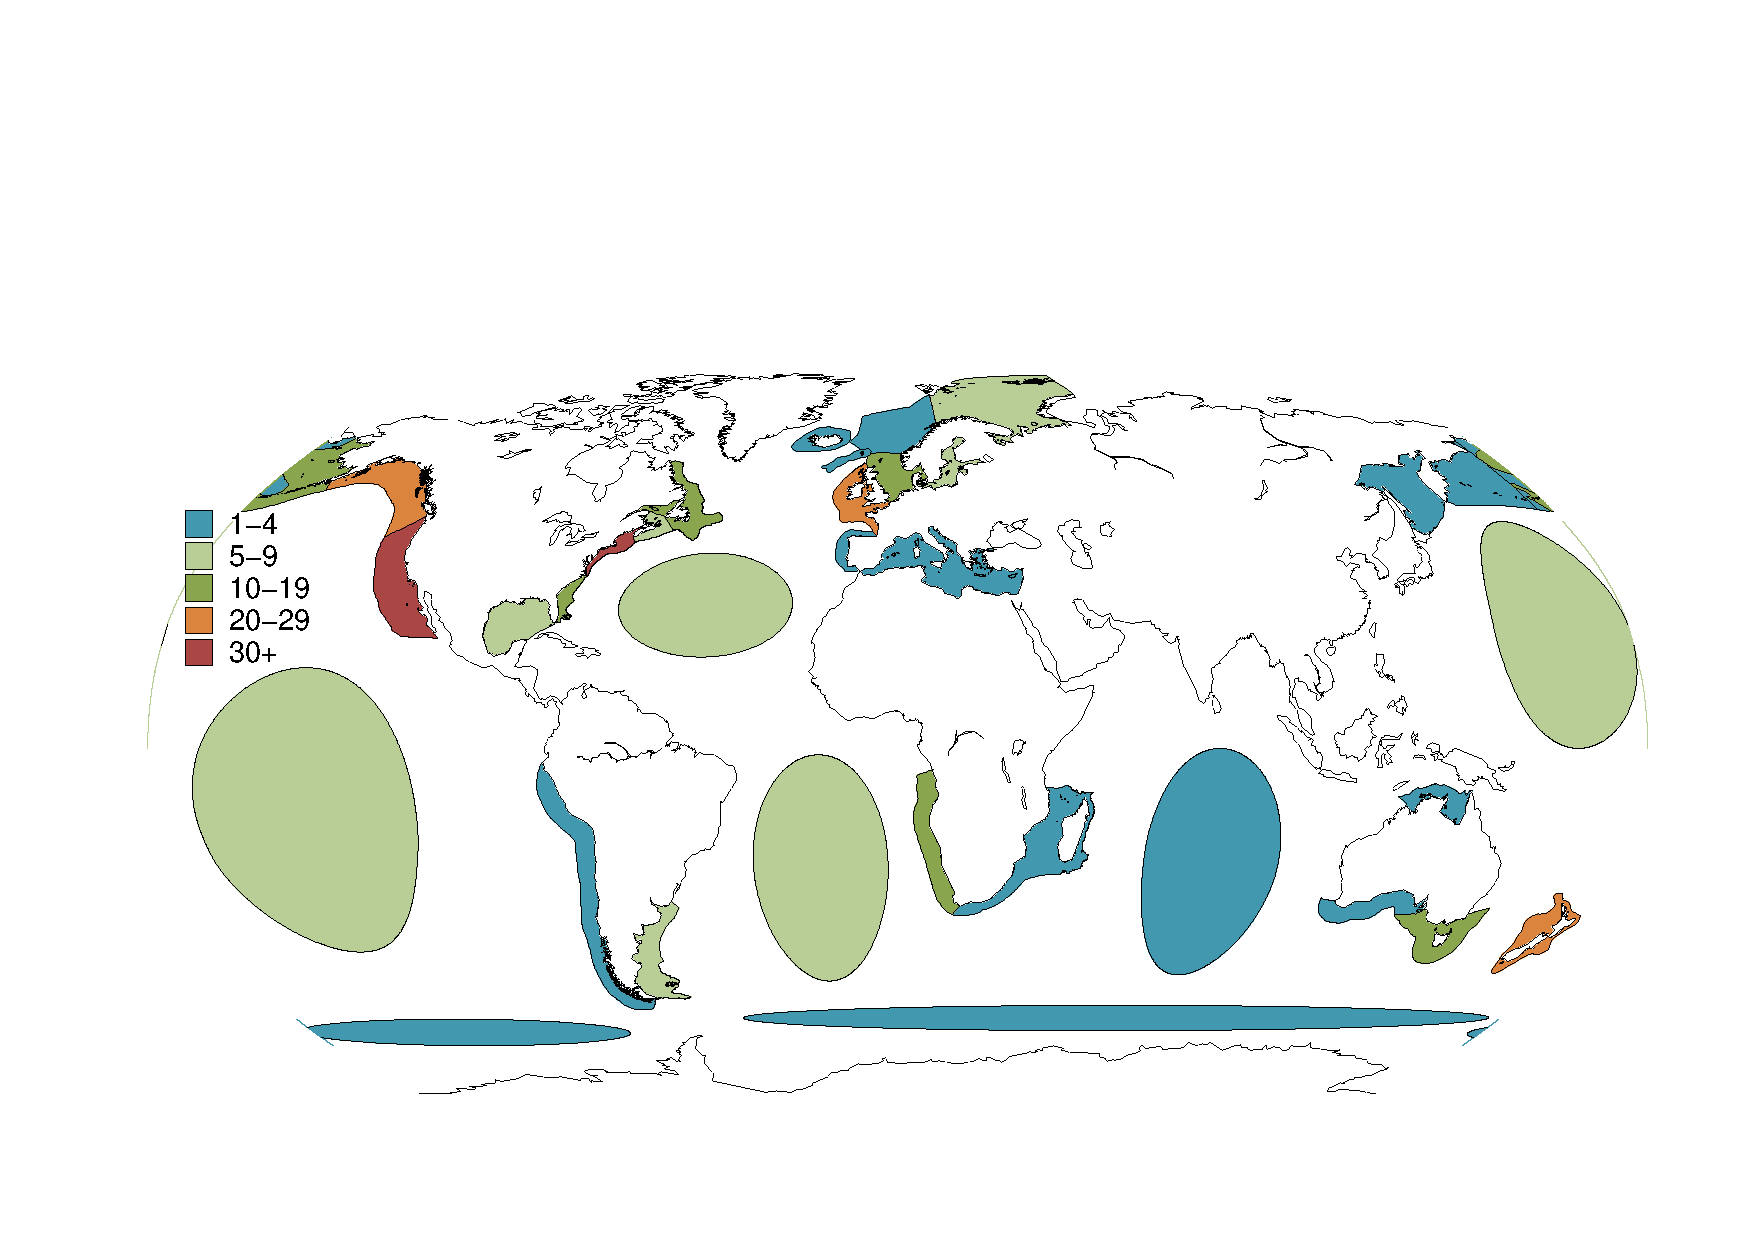
\includegraphics[width=15cm]{/home/srdbadmin/srdb/projects/fishandfisheries/GMT/stocks-byLME.pdf}
\end{center}
\caption{ }\label{fig:lmes}
\end{figure}

\begin{figure}
\begin{center}
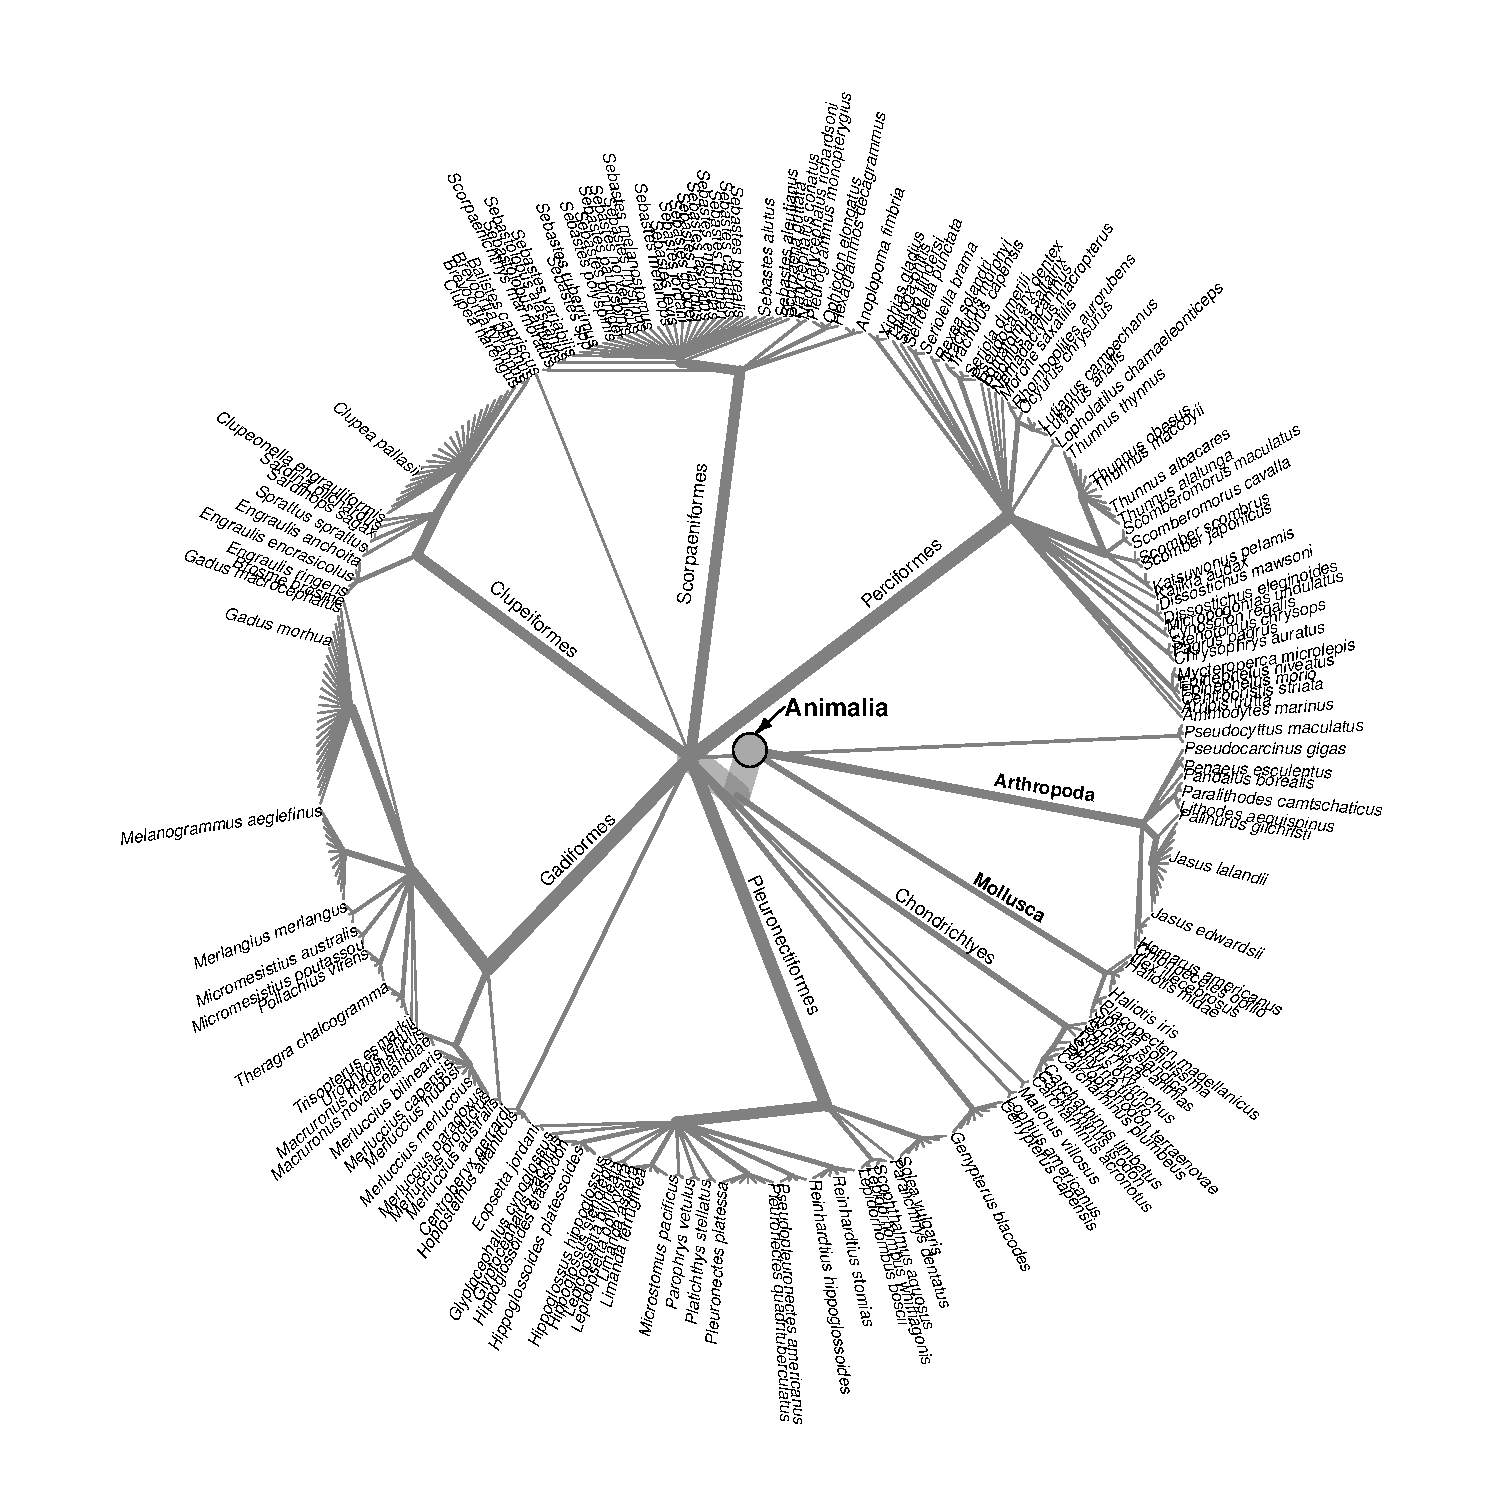
\includegraphics[width=15cm]{/home/srdbadmin/srdb/projects/fishandfisheries/R/srdb-by-assessment.pdf} %taxonomic_coverage_byLME.pdf}
\end{center}
\caption{ }\label{fig:taxo:srdb}
\end{figure}


\begin{figure}
\begin{center}
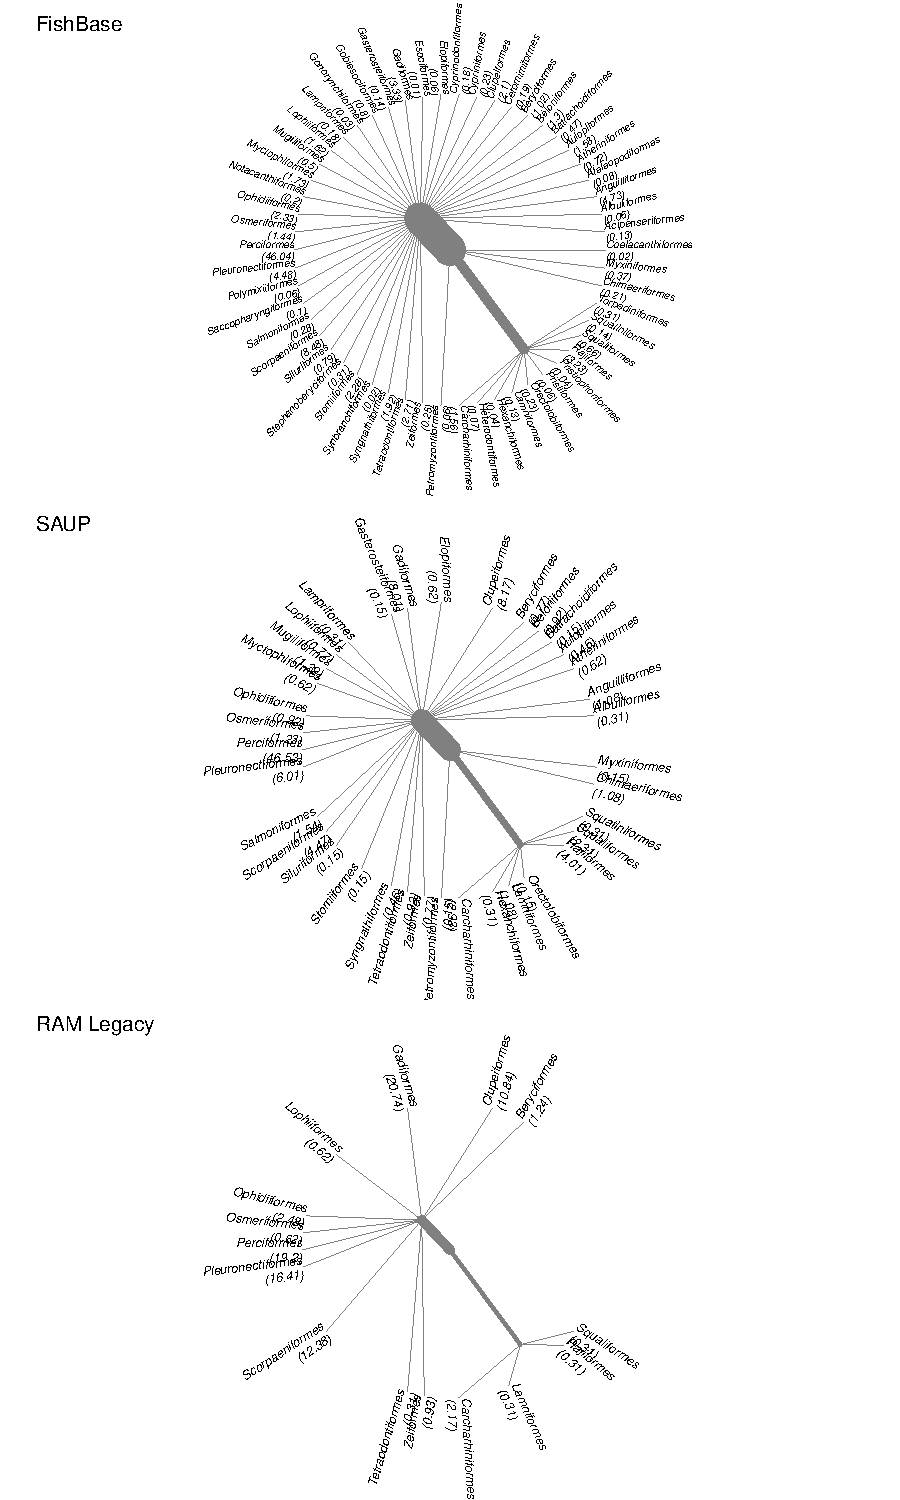
\includegraphics[width=12cm]{/home/srdbadmin/srdb/projects/fishandfisheries/R/three_panel_phylo.pdf} % fishbase_saup_two_panel_phylo.pdf}
\end{center}
\caption{ }\label{fig:taxo:threepanel}
\end{figure}

\begin{figure}
\begin{center}
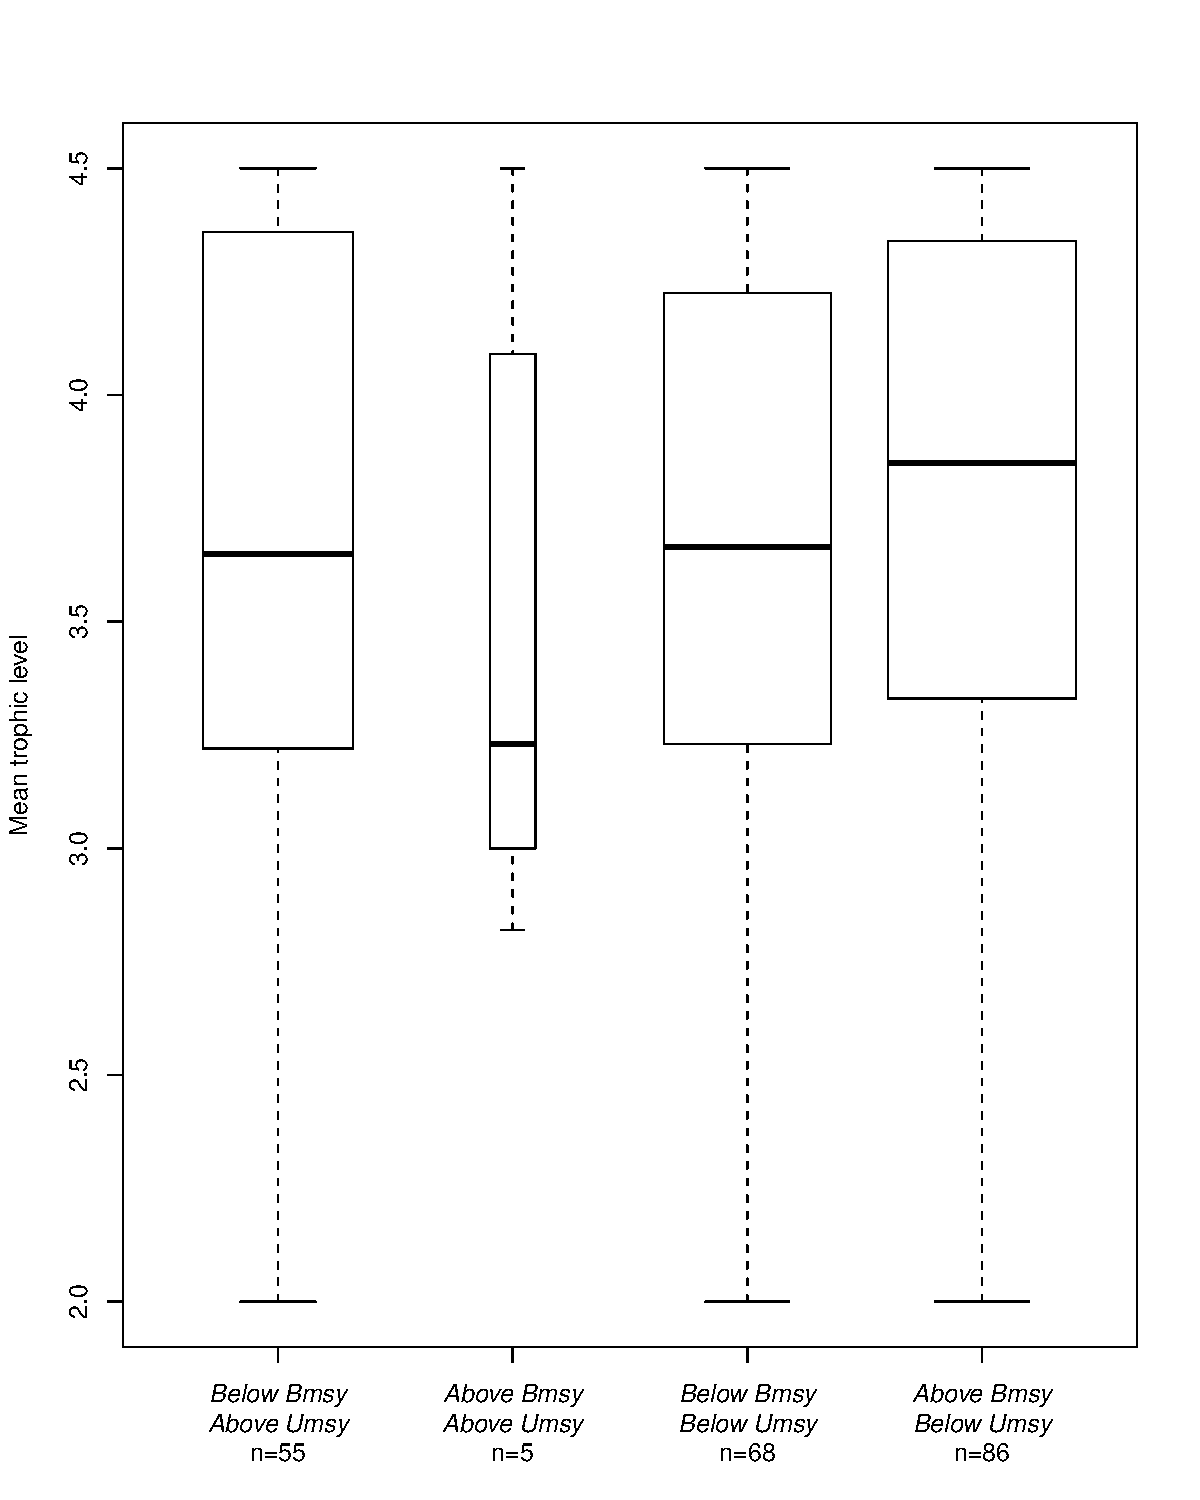
\includegraphics[width=15cm]{/home/srdbadmin/srdb/projects/fishandfisheries/R/TL-quadrant-srdb.pdf}
\end{center}
\caption{ }\label{fig:TL}
\end{figure}

\begin{figure}
\begin{center}
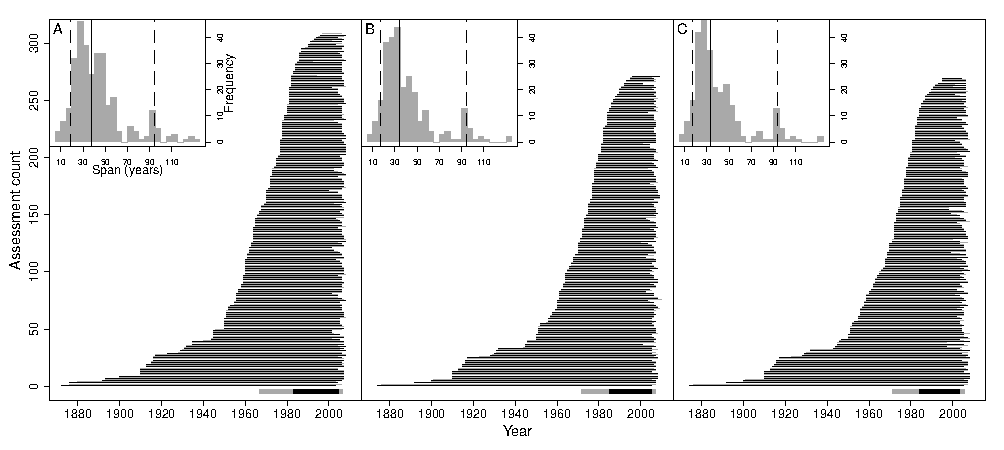
\includegraphics[width=15cm]{/home/srdbadmin/srdb/projects/fishandfisheries/R/orca_plot_v2.pdf}
\end{center}
\caption{ }\label{fig:orca}
\end{figure}

\begin{figure}
\begin{center}
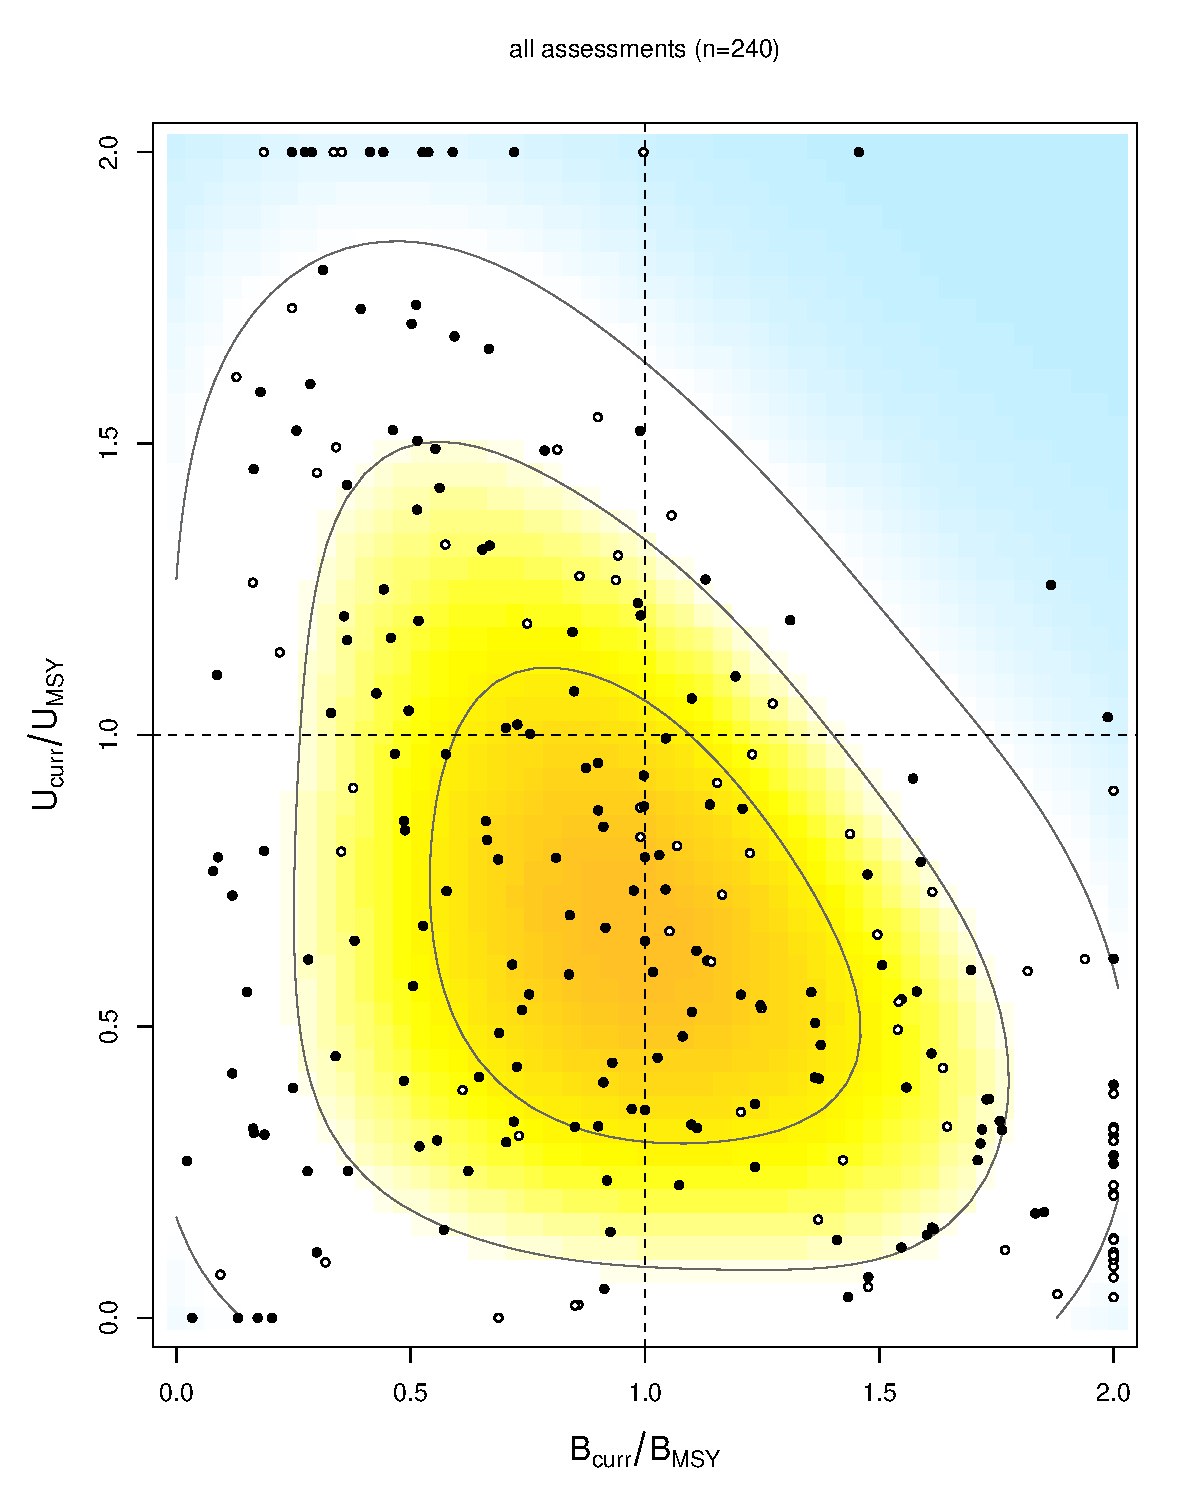
\includegraphics[width=15cm]{/home/srdbadmin/srdb/projects/fishandfisheries/R/friedegg-single.pdf}
\end{center}
\caption{ }\label{fig:friedegg}
\end{figure}

\begin{figure}
\begin{center}
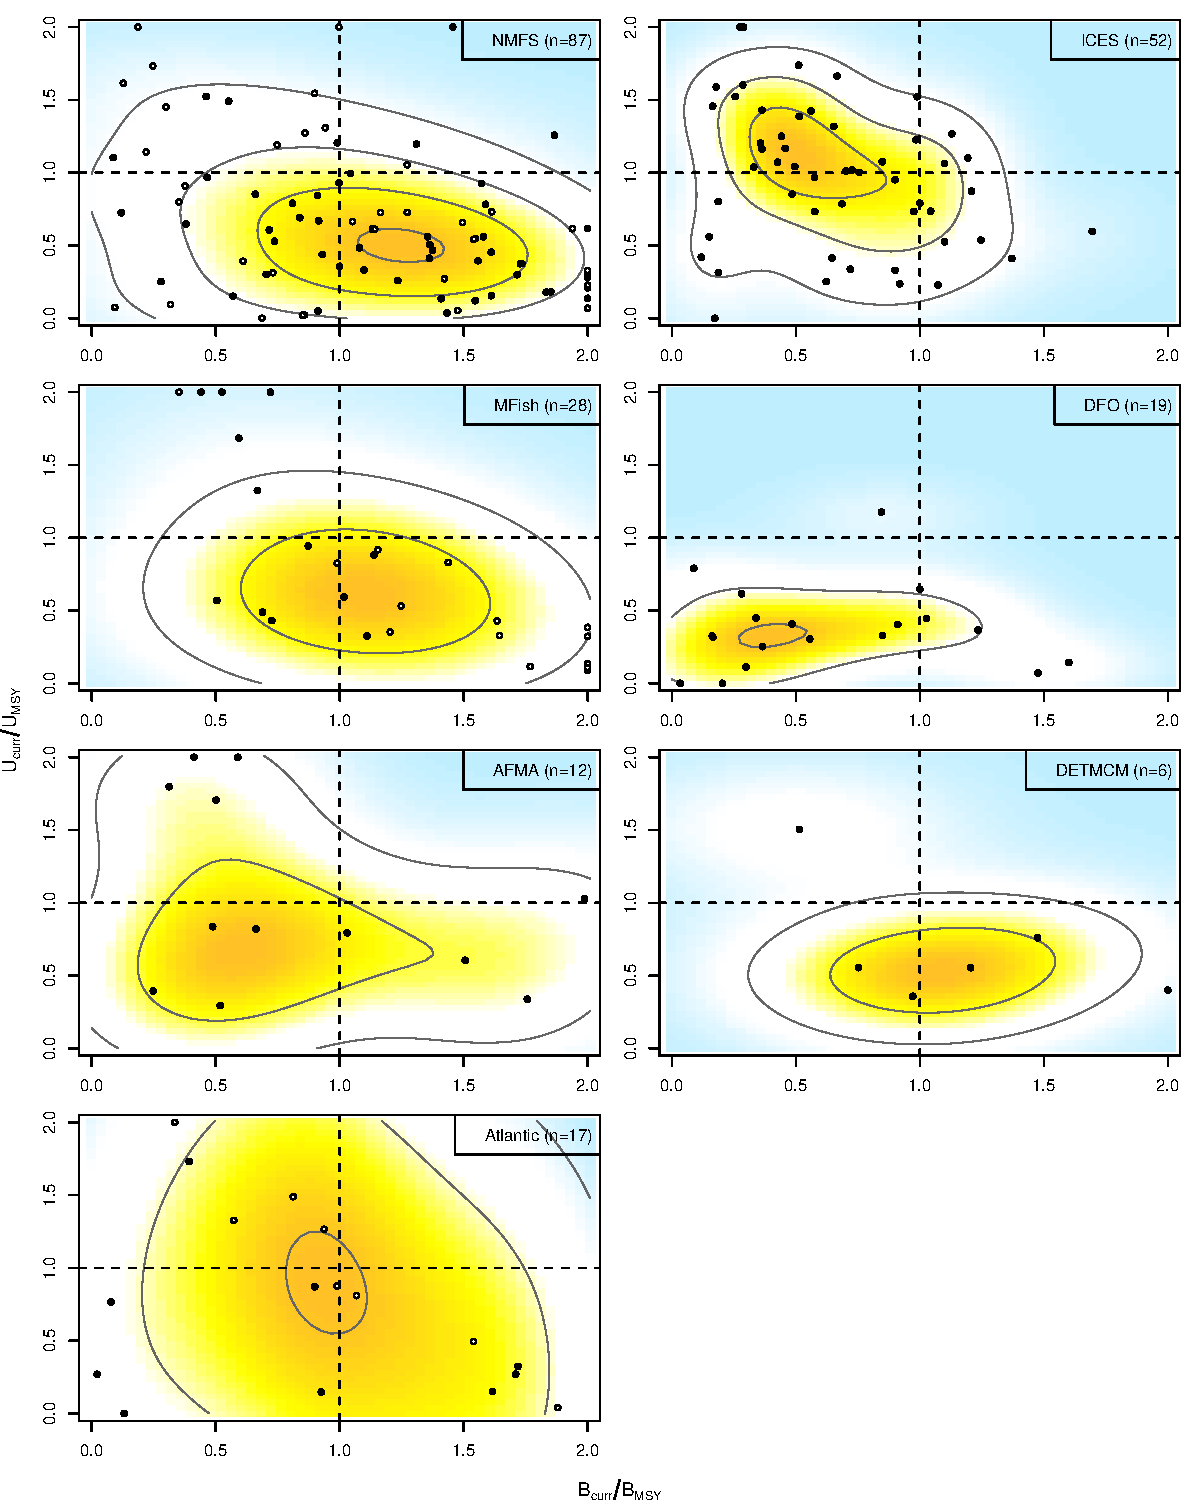
\includegraphics[width=15cm]{/home/srdbadmin/srdb/projects/fishandfisheries/R/friedegg-by-mgmt.pdf}
\end{center}
\caption{ }\label{fig:friedeggmgmt}
\end{figure}


\section*{Supporting Information}

\subsection*{Entity relationship diagram}
\begin{figure}
\begin{center}
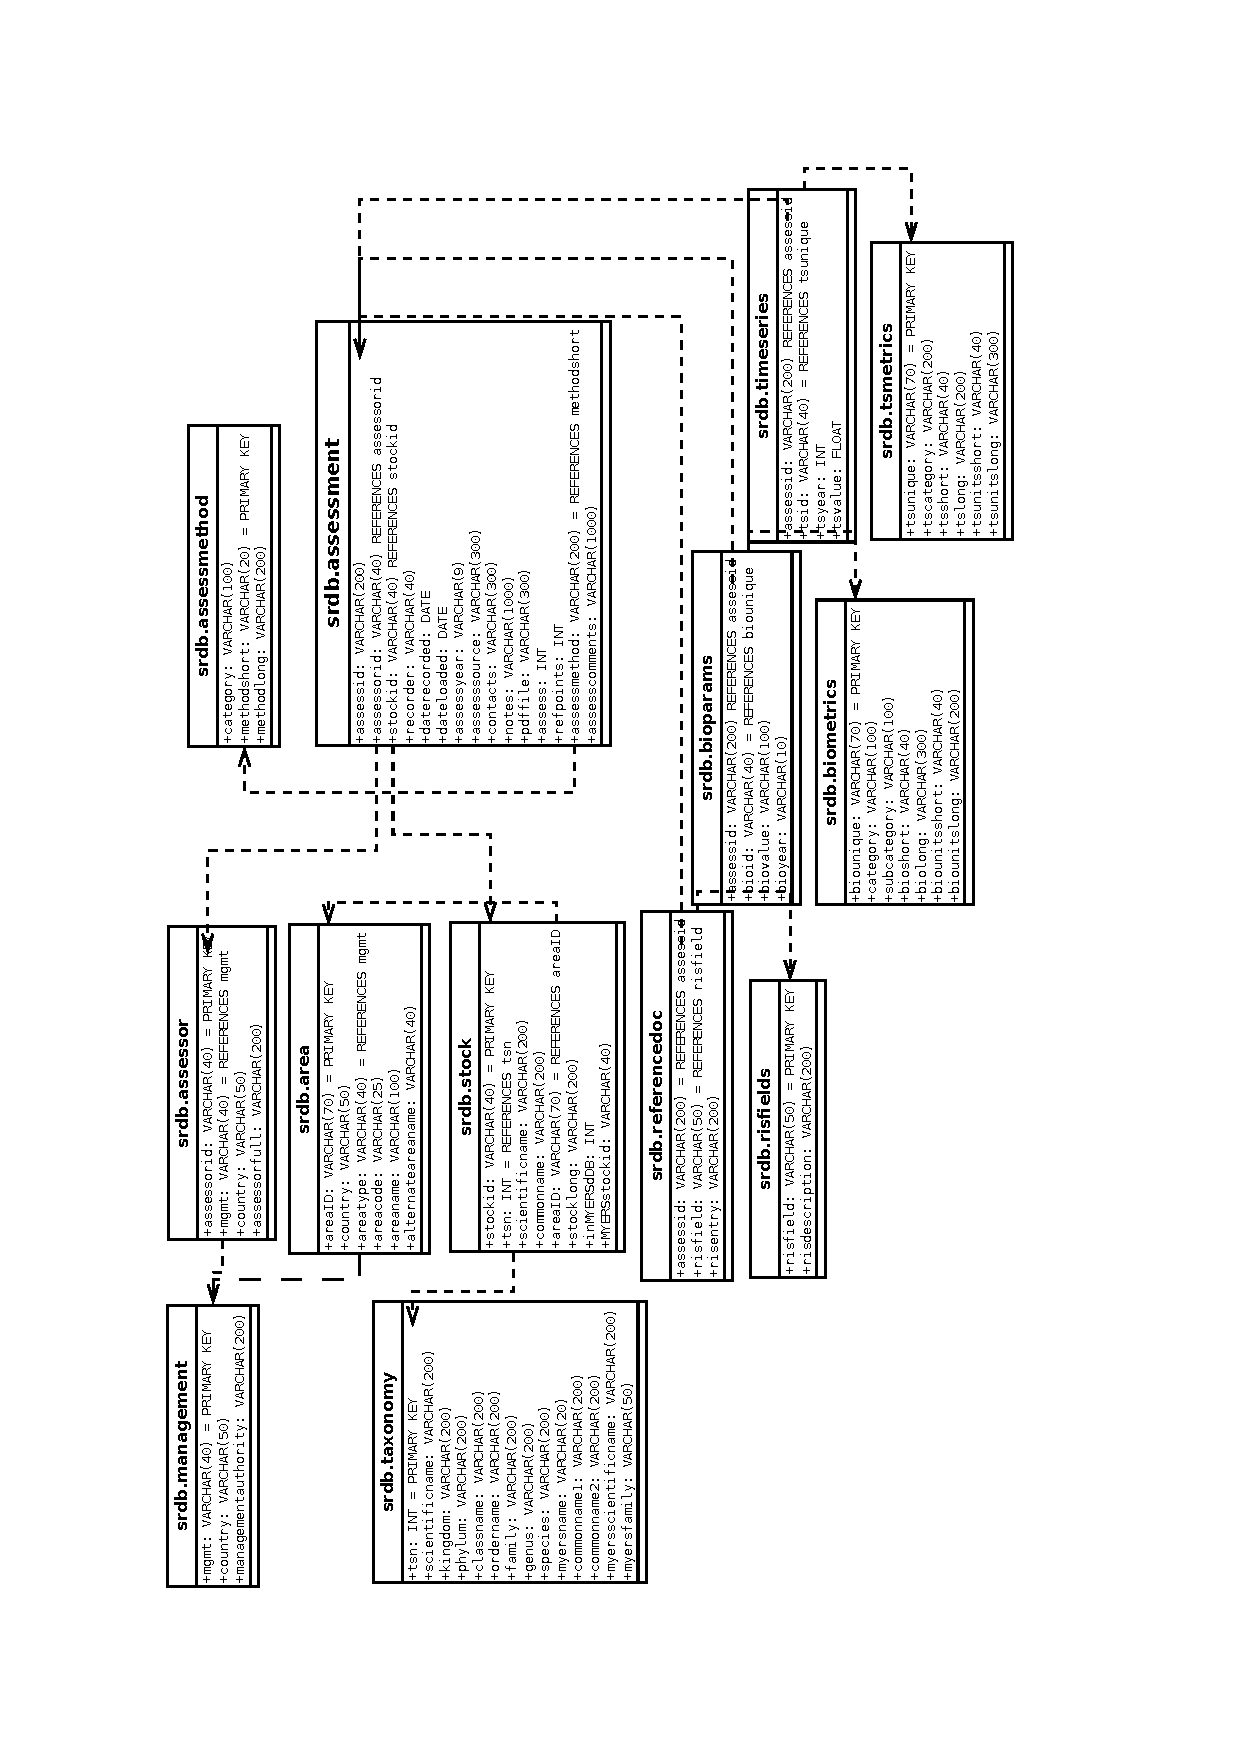
\includegraphics[width=15cm]{/home/srdbadmin/SQLpg/srdb/trunk/doc/srdb-ERD.pdf}
\end{center}
\caption{Entity relationship diagram of the RAM legacy database.}
\end{figure}


\begin{table}
\caption{Data used to generate Figure~\ref{fig:orca} - Summary of the assessments used in this analysis and the timespan of their different results. }
\begin{tabular}{| p{5cm} | p{3cm} | c | r  c  l | c | }\label{tab:timespan}
\textit{Fisheries stock} & \textit{Scientific name} & \textit{Timespan} & & \textit{Num. years available} & & \textit{Source} \\
 & & & Catch & SSB & R & \\
\hline \hline
blah & blah & 1970-2000 & 30 & 29 & 30 & (blah) \\
\end{tabular}
\end{table}


%\begin{table}
%\caption{Data used to generate Figures~\ref{fig:friedegg} and ~\ref{fig:friedeggmgmt} - Summary of the assessments used in this analysis and their estimated ratios of current biomass to the biomass at maximum sustainable yield and current harvest rate to the harvest rate that results is maximum sustainable yield. The estimated ratios were preferentially obtained directly from the assessment document or derived from surplus production model fits. When both an SSBmsy and Bmsy reference points are available, the SSB is chosen preferentially. }
%\begin{tabular}{| p{5cm} | p{3cm} | c | c | c | c | c |}\label{tab:crosshair}
%\textit{Fisheries stock} & \textit{Scientific name} & \textit{Current year} & \textit{B/Bmsy} & \textit{u/umsy} & \textit{From assessment?} & \textit{Source} \\
%\hline \hline
%blah & blah & 2000 & 1.0 & 1.0 & yes &  (blah) \\
%\end{tabular}
%\end{table}

% latex table generated in R 2.13.0 by xtable 1.5-6 package
% Thu May 19 14:38:14 2011
\begin{table}[ht]
\begin{center}
\begin{tabular}{ccc}
  \hline
 & SP U/Umsy $<$ 1 & SP U/Umsy $>$ 1 \\ 
  \hline
U/Umsy $<$ 1 &  20 &  14 \\ 
  U/Umsy $>$ 1 &   2 &   8 \\ 
  B/Bmsy $<$ 1 &  28 &   6 \\ 
  B/Bmsy $>$ 1 &  12 &  30 \\ 
   \hline
\end{tabular}
\caption{Contingency tables of stock status classification for biomass and exploitation reference points obtained from assessments and those derived from surplus production models. }
\label{tab:contingency}
\end{center}
\end{table}

\begin{table}[ht]
\begin{center}
\begin{tabular}{rllrrrl}
  \hline
 & stock & scientificname & currentyear & Bratio & Uratio & fromassessment \\
  \hline
1 & Alaska plaice Bering Sea and Aleutian Islands & Pleuronectes quadrituberculatus & 2008 & 2.46 & 0.05 & yes \\
  2 & Arrowtooth flounder Bering Sea and Aleutian Islands & Reinhardtius stomias & 2008 & 1.28 & 0.31 & no \\
  3 & Arrowtooth flounder Gulf of Alaska & Reinhardtius stomias & 2007 & 1.33 & 0.28 & no \\
  4 & Atka mackerel Bering Sea and Aleutian Islands & Pleurogrammus monopterygius & 2008 & 1.50 & 0.55 & no \\
  5 & Cabezon Northern California & Scorpaenichthys marmoratus & 2004 & 0.89 & 0.99 & no \\
  6 & Cabezon Southern California & Scorpaenichthys marmoratus & 2004 & 0.81 & 0.53 & no \\
  7 & Dusky rockfish Gulf of Alaska & Sebastes variabilis & 2007 & 1.54 & 0.54 & yes \\
  8 & Flathead sole Bering Sea and Aleutian Islands & Hippoglossoides elassodon & 2008 & 1.66 & 0.18 & no \\
  9 & Greenland turbot Bering Sea and Aleutian Islands & Reinhardtius hippoglossoides & 2009 & 1.48 & 0.05 & yes \\
  10 & Northern rockfish Bering Sea and Aleutian Islands & Sebastes polyspinis & 2008 & 1.07 & 0.13 & no \\
  11 & Northern rockfish Gulf of Alaska & Sebastes polyspinis & 2008 & 1.50 & 0.66 & yes \\
  12 & Northern rock sole Eastern Bering Sea and Aleutian Islands & Lepidopsetta polyxystra & 2007 & 3.02 & 0.21 & yes \\
  13 & Pacific cod Bering Sea and Aleutian Islands & Gadus macrocephalus & 2007 & 0.89 & 0.93 & no \\
  14 & Pacific cod Gulf of Alaska & Gadus macrocephalus & 2007 & 1.07 & 0.84 & no \\
  15 & Pacific Ocean perch Eastern Bering Sea and Aleutian Islands & Sebastes alutus & 2008 & 1.70 & 0.26 & no \\
  16 & Pacific ocean perch Gulf of Alaska & Sebastes alutus & 2008 & 1.16 & 0.73 & yes \\
  17 & Red king crab Bristol Bay & Paralithodes camtschaticus & 2007 & 0.00 & 1.38 & no \\
  18 & Sablefish Eastern Bering Sea / Aleutian Islands / Gulf of Alaska & Anoplopoma fimbria & 2008 & 0.72 & 0.90 & no \\
  19 & Snow crab Bering Sea & Chionoecetes opilio & 2008 & 0.29 & 1.61 & no \\
  20 & Walleye pollock Aleutian Islands & Theragra chalcogramma & 2008 & 0.86 & 0.02 & yes \\
  21 & Walleye pollock Eastern Bering Sea & Theragra chalcogramma & 2008 & 0.68 & 0.85 & no \\
  22 & Yellowfin sole Bering Sea and Aleutian Islands & Limanda aspera & 2008 & 1.94 & 0.62 & yes \\
  23 & Capelin Barents Sea & Mallotus villosus & 2006 & 0.17 & 0.00 & no \\
  24 & Atlantic cod coastal Norway & Gadus morhua & 2006 & 0.20 & 2.57 & no \\
  25 & Atlantic cod Northeast Arctic & Gadus morhua & 2006 & 0.56 & 1.42 & no \\
  26 & Greenland halibut Northeast Arctic & Reinhardtius hippoglossoides & 2006 & 0.23 & 1.38 & no \\
  27 & Golden Redfish Northeast Arctic & Sebastes norvegicus & 2006 & 0.00 & 4.25 & no \\
  28 & Haddock Northeast Arctic & Melanogrammus aeglefinus & 2006 & 1.10 & 1.06 & no \\
  29 & Pollock Northeast Arctic & Pollachius virens & 2006 & 1.70 & 0.60 & no \\
  30 & Atlantic croaker Mid-Atlantic Coast & Micropogonias undulatus & 2002 & 1.42 & 0.27 & yes \\
  31 & Northern shrimp Gulf of Maine & Pandalus borealis & 2008 & 1.58 & 0.56 & no \\
  32 & Antarctic toothfish Ross Sea & Dissostichus mawsoni & 2007 & 1.76 & 1.09 & no \\
  33 & Deepwater flathead Southeast Australia & Platycephalus conatus & 2006 & 1.33 & 0.61 & no \\
  34 & common gemfish Southeast Australia & Rexea solandri & 2007 & 0.01 & 0.59 & no \\
  35 & Jackass morwong Southeast Australia & Nemadactylus macropterus & 2007 & 0.25 & 1.80 & no \\
  36 & New Zealand ling Eastern half of Southeast Australia & Genypterus blacodes & 2007 & 0.60 & 2.20 & no \\
  37 & Orange roughy Cascade Plateau & Hoplostethus atlanticus & 2006 & 1.76 & 0.34 & no \\
  38 & Orange roughy Southeast Australia & Hoplostethus atlanticus & 2006 & 0.89 & 0.29 & no \\
  39 & Silverfish Southeast Australia & Seriolella punctata & 2006 & 1.15 & 0.79 & no \\
  40 & School whiting Southeast Australia & Sillago flindersi & 2007 & 1.10 & 0.82 & no \\
  41 & Tiger flathead Southeast Australia & Neoplatycephalus richardsoni & 2006 & 1.05 & 0.00 & no \\
  42 & Blue Warehou Eastern half of Southeast Australia & Seriolella brama & 2006 & 0.17 & 0.84 & no \\
  43 & Blue Warehou Western half of Southeast Australia & Seriolella brama & 2006 & 0.62 & 2.04 & no \\
  44 & Atlantic cod NAFO 5Zjm & Gadus morhua & 2002 & 0.00 & 0.74 & no \\
  45 & Haddock NAFO-4X5Y & Melanogrammus aeglefinus & 2003 & 0.28 & 0.45 & no \\
  46 & Haddock NAFO-5Zejm & Melanogrammus aeglefinus & 2002 & 0.15 & 0.86 & no \\
  47 & Atlantic cod NAFO 2J3KL inshore & Gadus morhua & 2005 & 1.60 & 0.14 & no \\
  48 & Atlantic cod NAFO 3Ps & Gadus morhua & 2004 & 0.43 & 0.43 & no \\
  49 & English sole Hecate Strait & Parophrys vetulus & 2001 & 1.23 & 0.37 & no \\
  50 & Pacific herring Central Coast & Clupea pallasii & 2007 & 0.30 & 0.11 & no \\
  51 & Pacific herring Prince Rupert District & Clupea pallasii & 2007 & 0.00 & 0.44 & no \\
  52 & Pacific herring Queen Charlotte Islands & Clupea pallasii & 2007 & 0.20 & 0.00 & no \\
  53 & Pacific herring Straight of Georgia & Clupea pallasii & 2007 & 0.91 & 0.40 & no \\
  54 & Pacific herring West Coast of Vancouver Island & Clupea pallasii & 2007 & 0.03 & 0.00 & no \\
  55 & Pacific cod Hecate Strait & Gadus macrocephalus & 2004 & 0.37 & 0.25 & no \\
  56 & Pacific cod West Coast of Vancouver Island & Gadus macrocephalus & 2001 & 0.28 & 0.61 & no \\
  57 & Rock sole Hecate Strait & Lepidopsetta bilineata & 2001 & 1.03 & 0.45 & no \\
  58 & Pollock NAFO-4VWX5Zc & Pollachius virens & 2006 & 0.56 & 0.30 & no \\
  59 & Atlantic cod NAFO 3Pn4RS & Gadus morhua & 2006 & 0.03 & 1.09 & no \\
  60 & Atlantic cod NAFO 4TVn & Gadus morhua & 2006 & 0.17 & 0.32 & no \\
  61 & Herring ICES 22-24-IIIa & Clupea harengus & 2006 & 0.73 & 1.02 & no \\
  62 & Herring Northern Irish Sea & Clupea harengus & 2006 & 0.72 & 0.34 & no \\
  63 & Herring North Sea & Clupea harengus & 2006 & 0.65 & 1.32 & no \\
  64 & Herring ICES VIa & Clupea harengus & 2006 & 0.18 & 1.59 & no \\
  65 & Herring ICES VIa-VIIb-VIIc & Clupea harengus & 2000 & 0.50 & 1.04 & no \\
  66 & Albacore tuna North Atlantic & Thunnus alalunga & 2005 & 0.81 & 1.49 & yes \\
  67 & Bluefin tuna Eastern Atlantic & Thunnus thynnus & 2007 & 0.34 & 9.38 & yes \\
  68 & Bluefin tuna Western Atlantic & Thunnus thynnus & 2007 & 0.57 & 1.33 & yes \\
  69 & Bigeye tuna Atlantic & Thunnus obesus & 2005 & 0.90 & 0.86 & no \\
  70 & Skipjack tuna Eastern Atlantic & Katsuwonus pelamis & 2006 & 1.71 & 0.27 & no \\
  71 & Skipjack tuna Western Atlantic & Katsuwonus pelamis & 2006 & 1.72 & 0.27 & no \\
  72 & Swordfish Mediterranean Sea & Xiphias gladius & 2006 & 0.94 & 1.27 & yes \\
  73 & Swordfish North Atlantic & Xiphias gladius & 2005 & 1.03 & 0.82 & no \\
  74 & Swordfish South Atlantic & Xiphias gladius & 2005 & 1.18 & 0.69 & no \\
  75 & Yellowfin tuna Atlantic & Thunnus albacares & 2006 & 1.07 & 0.81 & yes \\
  76 & Chilean jack mackerel Chilean EEZ and offshore & Trachurus murphyi & 2006 & 0.52 & 1.20 & no \\
  77 & Argentine anchoita Northern Argentina & Engraulis anchoita & 2007 & 1.37 & 0.17 & yes \\
  78 & Argentine anchoita Southern Argentina & Engraulis anchoita & 2007 & 3.13 & 0.04 & yes \\
  79 & Argentine hake Northern Argentina & Merluccius hubbsi & 2007 & 0.16 & 1.26 & yes \\
  80 & Argentine hake Southern Argentina & Merluccius hubbsi & 2008 & 0.34 & 1.49 & yes \\
  81 & Patagonian grenadier Southern Argentina & Macruronus magellanicus & 2006 & 1.82 & 0.60 & yes \\
  82 & Bigeye tuna Indian Ocean & Thunnus obesus & 2004 & 1.23 & 0.97 & yes \\
  83 & Pacific halibut North Pacific & Hippoglossus stenolepis & 2008 & 0.54 & 2.01 & no \\
  84 & Anchovy South Africa & Engraulis encrasicolus & 2006 & 0.97 & 0.36 & no \\
  85 & Shallow-water cape hake South Africa & Merluccius capensis & 2008 & 1.16 & 0.40 & no \\
  86 & Cape horse mackerel South Africa South coast & Trachurus capensis & 2007 & 1.47 & 0.76 & no \\
  87 & Kingklip South Africa & Engraulis encrasicolus & 2008 & 1.13 & 0.55 & no \\
  88 & Sardine South Africa & Sardinops sagax & 2006 & 0.75 & 0.55 & no \\
  89 & Southern spiny lobster South Africa South coast & Palinurus gilchristi & 2008 & 0.51 & 1.50 & no \\
  90 & American Plaice NAFO-3LNO & Hippoglossoides platessoides & 2006 & 0.02 & 1.05 & no \\
  91 & American Plaice NAFO-3M & Hippoglossoides platessoides & 2007 & 0.00 & 0.00 & no \\
  92 & Atlantic cod NAFO 3NO & Gadus morhua & 2006 & 0.00 & 0.38 & no \\
  93 & Greenland halibut NAFO 23KLMNO & Reinhardtius hippoglossoides & 2006 & 0.39 & 1.73 & no \\
  94 & Redfish species NAFO 3LN & Redfish species & 2008 & 1.88 & 0.04 & yes \\
  95 & Redfish species NAFO 3M & Redfish species & 2006 & 0.93 & 0.15 & no \\
  96 & Yellowtail Flounder NAFO 3LNO & Limanda ferruginea & 2007 & 1.62 & 0.15 & no \\
  97 & American Plaice NAFO-5YZ & Hippoglossoides platessoides & 2007 & 0.55 & 0.30 & no \\
  98 & Bluefish Atlantic Coast & Pomatomus saltatrix & 2007 & 0.81 & 1.25 & no \\
  99 & Black sea bass Mid-Atlantic Coast & Centropristis striata & 2007 & 1.21 & 0.67 & no \\
  100 & Atlantic cod Georges Bank & Gadus morhua & 2007 & 0.00 & 1.15 & no \\
  101 & Atlantic cod Gulf of Maine & Gadus morhua & 2007 & 1.46 & 0.29 & no \\
  102 & Haddock NAFO-5Y & Melanogrammus aeglefinus & 2007 & 0.00 & 1.86 & no \\
  103 & Monkfish Gulf of Maine / Northern Georges Bank & Lophius americanus & 2006 & 1.73 & 0.38 & no \\
  104 & Monkfish Southern Georges Bank / Mid-Atlantic & Lophius americanus & 2006 & 1.72 & 0.30 & no \\
  105 & Sea scallop Georges Bank & Placopecten magellanicus & 2006 & 1.59 & 0.78 & no \\
  106 & Sea scallop Mid-Atlantic Coast & Placopecten magellanicus & 2006 & 0.91 & 0.37 & no \\
  107 & Spiny dogfish Atlantic Coast & Squalus acanthias & 2005 & 1.61 & 0.15 & no \\
  108 & Atlantic surfclam Mid-Atlantic Coast & Spisula solidissima & 1994 & 1.85 & 0.00 & no \\
  109 & Tilefish Mid-Atlantic Coast & Lopholatilus chamaeleonticeps & 2005 & 0.72 & 0.61 & no \\
  110 & Weakfish Atlantic Coast & Cynoscion regalis & 2008 & 0.06 & 1.49 & no \\
  111 & White hake Georges Bank / Gulf of Maine & Urophycis tenuis & 2007 & 0.35 & 0.80 & yes \\
  112 & Winter Flounder NAFO-5Z & Pseudopleuronectes americanus & 2006 & 1.41 & 0.25 & no \\
  113 & Winter Flounder Southern New England-Mid Atlantic & Pseudopleuronectes americanus & 2007 & 0.07 & 1.44 & no \\
  114 & Witch Flounder NAFO-5Y & Glyptocephalus cynoglossus & 2007 & 0.30 & 1.45 & yes \\
  115 & Yellowtail flounder Cape Cod / Gulf of Maine & Limanda ferruginea & 2007 & 0.25 & 1.73 & yes \\
  116 & Yellowtail flounder Georges Bank & Limanda ferruginea & 2007 & 0.22 & 1.14 & yes \\
  117 & Yellowtail Flounder Southern New England-Mid Atlantic & Limanda ferruginea & 2007 & 0.13 & 1.61 & yes \\
  118 & Australian salmon New Zealand & Arripis trutta & 2006 & 1.64 & 0.33 & yes \\
  119 & Orange roughy New Zealand Mid East Coast & Hoplostethus atlanticus & 2004 & 1.20 & 0.35 & yes \\
  120 & Atlantic menhaden Atlantic & Brevoortia tyrannus & 2005 & 0.47 & 0.97 & no \\
  121 & Pacific sardine North Pacific & Sardinops sagax & 2006 & 1.73 & 0.37 & no \\
  122 & Arrowtooth flounder Pacific Coast & Reinhardtius stomias & 2007 & 3.81 & 0.21 & yes \\
  123 & Blackgill rockfish  Pacific Coast & Sebastes melanostomus & 2004 & 0.80 & 1.20 & no \\
  124 & Black rockfish Northern Pacific Coast & Sebastes melanops & 2006 & 1.37 & 0.57 & no \\
  125 & Black rockfish Southern Pacific Coast & Sebastes melanops & 2007 & 2.23 & 0.33 & yes \\
  126 & Blue rockfish California & Sebastes mystinus & 2007 & 0.75 & 1.19 & yes \\
  127 & Bocaccio Southern Pacific Coast & Sebastes paucispinis & 2006 & 0.32 & 0.10 & yes \\
  128 & Chilipepper Southern Pacific Coast & Sebastes goodei & 2006 & 1.43 & 0.04 & no \\
  129 & Cowcod Southern California & Sebastes levis & 2007 & 0.09 & 0.07 & yes \\
  130 & Canary rockfish Pacific Coast & Sebastes pinniger & 2007 & 0.85 & 0.02 & yes \\
  131 & Darkblotched rockfish Pacific Coast & Sebastes crameri & 2007 & 0.73 & 0.31 & yes \\
  132 & English sole Pacific Coast & Parophrys vetulus & 2006 & 2.06 & 0.14 & no \\
  133 & Longnose skate Pacific Coast & Raja rhina & 2007 & 1.56 & 0.40 & no \\
  134 & Longspine thornyhead Pacific Coast & Sebastolobus altivelis & 2005 & 2.65 & 0.23 & yes \\
  135 & Pacific hake Pacific Coast & Merluccius productus & 2007 & 0.42 & 1.67 & no \\
  136 & Pacific ocean perch Pacific Coast & Sebastes alutus & 2007 & 0.69 & 0.00 & yes \\
  137 & Petrale sole Northern Pacific Coast & Eopsetta jordani & 2004 & 0.96 & 1.26 & no \\
  138 & Petrale sole Southern Pacific Coast & Eopsetta jordani & 2004 & 0.63 & 0.61 & no \\
  139 & Sablefish Pacific Coast & Anoplopoma fimbria & 2007 & 0.84 & 1.09 & no \\
  140 & Shortspine thornyhead Pacific Coast & Sebastolobus alascanus & 2004 & 1.55 & 0.93 & no \\
  141 & Widow rockfish Pacific Coast & Sebastes entomelas & 2006 & 0.91 & 0.07 & no \\
  142 & Yelloweye rockfish Pacific Coast & Sebastes ruberrimus & 2006 & 0.38 & 0.34 & no \\
  143 & Yellowtail rockfish Northern Pacific Coast & Sebastes flavidus & 2005 & 0.75 & 0.51 & no \\
  144 & Capelin Iceland & Mallotus villosus & 2006 & 0.49 & 0.85 & no \\
  145 & Atlantic cod Faroe Plateau & Gadus morhua & 2006 & 0.26 & 1.52 & no \\
  146 & Atlantic cod Iceland & Gadus morhua & 2006 & 0.46 & 1.17 & no \\
  147 & Haddock Faroe Plateau & Melanogrammus aeglefinus & 2006 & 0.85 & 1.07 & no \\
  148 & Haddock Iceland & Melanogrammus aeglefinus & 2007 & 0.73 & 1.36 & no \\
  149 & Pollock Faroe Plateau & Pollachius virens & 2006 & 0.99 & 1.52 & no \\
  150 & Black oreo West end of Chatham Rise & Allocyttus niger & 2007 & 0.99 & 0.82 & yes \\
  151 & Smooth oreo Chatham Rise & Pseudocyttus maculatus & 2006 & 2.25 & 0.38 & yes \\
  152 & Smooth oreo West end of Chatham Rise & Pseudocyttus maculatus & 2004 & 1.25 & 0.53 & yes \\
  153 & Hoki Eastern New Zealand & Macruronus novaezelandiae & 2007 & 1.11 & 0.33 & no \\
  154 & Hoki Western New Zealand & Macruronus novaezelandiae & 2007 & 0.51 & 0.57 & no \\
  155 & New Zealand snapper New Zealand Area 8 & Chrysophrys auratus & 2005 & 0.35 & 2.50 & yes \\
  156 & Trevally New Zealand Areas TRE 7 & Pseudocaranx dentex & 2005 & 1.44 & 0.83 & yes \\
  157 & Red rock lobster New Zealand area CRA1 & Jasus edwardsii & 2001 & 1.14 & 0.88 & no \\
  158 & Red rock lobster New Zealand area CRA2 & Jasus edwardsii & 2001 & 0.53 & 2.12 & no \\
  159 & Red rock lobster New Zealand area CRA4 & Jasus edwardsii & 2005 & 0.67 & 1.33 & no \\
  160 & Red rock lobster New Zealand area CRA5 & Jasus edwardsii & 2002 & 0.59 & 1.68 & no \\
  161 & Red rock lobster New Zealand area CRA7 & Jasus edwardsii & 2005 & 0.73 & 0.43 & no \\
  162 & Red rock lobster New Zealand area CRA8 & Jasus edwardsii & 2005 & 0.69 & 0.49 & no \\
  163 & common gemfish New Zealand & Rexea solandri & 2006 & 1.64 & 0.43 & yes \\
  164 & New Zealand ling New Zealand Areas LIN 3 and 4 & Genypterus blacodes & 2007 & 3.07 & 0.09 & yes \\
  165 & New Zealand ling New Zealand Areas LIN 5 and 6 & Genypterus blacodes & 2007 & 3.96 & 0.10 & yes \\
  166 & New Zealand ling New Zealand Area LIN 6b & Genypterus blacodes & 2006 & 2.19 & 0.11 & yes \\
  167 & New Zealand ling New Zealand Area LIN 72 & Genypterus blacodes & 2007 & 2.49 & 0.32 & yes \\
  168 & New Zealand ling New Zealand Area LIN 7WC - WCSI & Genypterus blacodes & 2008 & 2.21 & 0.13 & yes \\
  169 & Southern blue whiting Campbell Island Rise & Micromesistius australis & 2006 & 1.15 & 0.92 & yes \\
  170 & Southern hake Chatham Rise & Merluccius australis & 2006 & 1.77 & 0.12 & yes \\
  171 & Southern hake Sub-Antarctic & Merluccius australis & 2007 & 2.91 & 0.11 & yes \\
  172 & New Zealand abalone species New Zealand Area PAU 5A & Haliotis iris & 2006 & 0.72 & 2.83 & no \\
  173 & New Zealand abalone species New Zealand Area PAU 5B & Haliotis iris & 2007 & 1.02 & 0.59 & no \\
  174 & New Zealand abalone species New Zealand Area PAU 5D & Haliotis iris & 2006 & 0.44 & 2.10 & no \\
  175 & New Zealand abalone species New Zealand Area PAU 7 & Haliotis iris & 2008 & 0.87 & 0.94 & no \\
  176 & American lobster Rhode Island & Homarus americanus & 2006 & 0.51 & 0.68 & no \\
  177 & Tautog Rhode Island & Tautoga onitis & 2006 & 0.84 & 0.59 & no \\
  178 & Winter flounder Rhode Island & Pseudopleuronectes americanus & 2006 & 0.03 & 2.35 & no \\
  179 & Gag Gulf of Mexico & Mycteroperca microlepis & 2004 & 1.25 & 1.84 & no \\
  180 & Gag Southern Atlantic coast & Mycteroperca microlepis & 2005 & 0.94 & 1.31 & yes \\
  181 & Greater amberjack Gulf of Mexico & Seriola dumerili & 2004 & 0.46 & 1.52 & no \\
  182 & King mackerel Gulf of Mexico & Scomberomorus cavalla & 2001 & 1.51 & 0.44 & no \\
  183 & King mackerel Southern Atlantic Coast & Scomberomorus cavalla & 2001 & 1.38 & 0.56 & no \\
  184 & Gulf menhaden Gulf of Mexico & Brevoortia patronus & 2004 & 1.08 & 0.48 & no \\
  185 & Red grouper Gulf of Mexico & Epinephelus morio & 2005 & 0.17 & 1.39 & no \\
  186 & Red porgy Southern Atlantic coast & Pagrus pagrus & 2004 & 0.61 & 0.39 & yes \\
  187 & Snowy grouper Southern Atlantic coast & Epinephelus niveatus & 2002 & 0.19 & 3.08 & yes \\
  188 & Spanish mackerel Southern Atlantic Coast & Scomberomorus maculatus & 2007 & 0.38 & 0.91 & yes \\
  189 & Tilefish Southern Atlantic coast & Lopholatilus chamaeleonticeps & 2002 & 0.94 & 1.55 & yes \\
  190 & Vermilion snapper Southern Atlantic coast & Rhomboplites aurorubens & 2007 & 0.86 & 1.27 & yes \\
  191 & Yellowtail snapper Southern Atlantic Coast and Gulf of Mexico & Ocyurus chrysurus & 2001 & 1.14 & 0.61 & yes \\
  192 & Walleye pollock Northern Sea of Okhotsk & Theragra chalcogramma & 1992 & 1.11 & 0.87 & no \\
  193 & Albacore tuna South Pacific Ocean & Thunnus alalunga & 2006 & 2.46 & 0.90 & yes \\
  194 & Bigeye tuna Western Pacific Ocean & Thunnus obesus & 2006 & 1.06 & 1.38 & yes \\
  195 & Skipjack tuna Central Western Pacific & Katsuwonus pelamis & 2006 & 4.38 & 0.30 & yes \\
  196 & Yellowfin tuna Central Western Pacific & Thunnus albacares & 2005 & 1.22 & 0.80 & yes \\
  197 & Dover sole Pacific Coast & Microstomus pacificus & 2004 & 1.33 & 0.45 & no \\
  198 & Gopher rockfish Southern Pacific Coast & Sebastes carnatus & 2004 & 1.69 & 0.08 & no \\
  199 & Pacific sardine Pacific Coast & Sardinops sagax & 2006 & 1.36 & 0.41 & no \\
  200 & Starry flounder Northern Pacific Coast & Platichthys stellatus & 2004 & 0.68 & 0.33 & no \\
  201 & Starry flounder Southern Pacific Coast & Platichthys stellatus & 2004 & 1.15 & 0.12 & no \\
  202 & Tasmanian giant crab Tasmania & Pseudocarcinus gigas & 2007 & 0.50 & 1.71 & no \\
  203 & Walleye pollock Western Bering Sea & Theragra chalcogramma & 2004 & 2.16 & 0.26 & no \\
  204 & Atlantic cod Baltic Areas 22 and 24 & Gadus morhua & 2006 & 0.31 & 1.55 & no \\
  205 & Atlantic cod Baltic Areas 25-32 & Gadus morhua & 2006 & 0.14 & 1.58 & no \\
  206 & Atlantic cod Kattegat & Gadus morhua & 2006 & 0.19 & 0.31 & no \\
  207 & Herring ICES 25-32 & Clupea harengus & 2006 & 0.69 & 0.79 & no \\
  208 & Herring ICES 30 & Clupea harengus & 2006 & 1.19 & 1.10 & no \\
  209 & Herring ICES 31 & Clupea harengus & 2006 & 0.27 & 1.65 & no \\
  210 & Herring Iceland (Summer spawners) & Clupea harengus & 2006 & 0.70 & 0.89 & no \\
  211 & Herring ICES 28 & Clupea harengus & 2006 & 1.21 & 0.87 & no \\
  212 & common European sole ICES Kattegat and Skagerrak & Solea vulgaris & 2006 & 1.25 & 0.54 & no \\
  213 & Sprat ICES Baltic Areas 22-32 & Sprattus sprattus & 2006 & 1.13 & 1.27 & no \\
  214 & Fourspotted megrim ICES VIIIc-IXa & Lepidorhombus boscii & 2006 & 0.00 & 1.61 & no \\
  215 & Hake Northeast Atlantic North & Merluccius merluccius & 2006 & 1.04 & 0.74 & no \\
  216 & Megrim ICES VIIIc-IXa & Lepidorhombus whiffiagonis & 2006 & 0.24 & 1.31 & no \\
  217 & common European sole Bay of Biscay & Solea vulgaris & 2006 & 0.62 & 1.13 & no \\
  218 & Mackerel ICES Northeast Atlantic & Scomber scombrus & 2006 & 0.98 & 0.73 & no \\
  219 & Whiting Northeast Atlantic & Micromesistius poutassou & 2006 & 0.67 & 1.66 & no \\
  220 & Atlantic cod Irish Sea & Gadus morhua & 2006 & 0.09 & 0.69 & no \\
  221 & Atlantic cod West of Scotland & Gadus morhua & 2006 & 0.10 & 0.45 & no \\
  222 & Haddock West of Scotland & Melanogrammus aeglefinus & 2006 & 0.58 & 0.73 & no \\
  223 & European Plaice Irish Sea & Pleuronectes platessa & 2006 & 1.07 & 0.23 & no \\
  224 & common European sole Irish Sea & Solea vulgaris & 2006 & 0.36 & 1.16 & no \\
  225 & Atlantic cod North Sea & Gadus morhua & 2006 & 0.19 & 0.80 & no \\
  226 & Haddock ICES IIIa and North Sea & Melanogrammus aeglefinus & 2006 & 0.62 & 0.25 & no \\
  227 & Haddock Rockall Bank & Melanogrammus aeglefinus & 2006 & 1.10 & 0.52 & no \\
  228 & Norway pout North Sea & Trisopterus esmarkii & 2006 & 0.90 & 0.33 & no \\
  229 & Pollock ICES IIIa, VI and North Sea & Pollachius virens & 2006 & 0.56 & 0.97 & no \\
  230 & Sandeel North Sea & Ammodytes marinus & 2007 & 0.92 & 0.24 & no \\
  231 & Whiting ICES IIIa, VIId and North Sea & Merlangius merlangus & 2006 & 0.33 & 1.04 & no \\
  232 & Haddock ICES VIIb-k & Melanogrammus aeglefinus & 2006 & 1.37 & 0.41 & no \\
  233 & European Plaice ICES VIIf-g & Pleuronectes platessa & 2006 & 0.65 & 0.41 & no \\
  234 & European Plaice ICES VIIe & Pleuronectes platessa & 2006 & 0.51 & 1.39 & no \\
  235 & common European sole Celtic Sea & Solea vulgaris & 2006 & 0.90 & 0.95 & no \\
  236 & common European sole Western English Channel & Solea vulgaris & 2006 & 0.51 & 1.75 & no \\
  237 & Whiting ICES VIIe-k & Merlangius merlangus & 2006 & 0.44 & 1.25 & no \\
   \hline
\end{tabular}
\caption{Data used to generate Figures~\ref{fig:friedegg} and ~\ref{fig:friedeggmgmt} - Summary of the assessments used in this analysis and their estimated ratios of current biomass to the biomass at maximum sustainable yield and current harvest rate to the harvest rate that results is maximum sustainable yield. The estimated ratios were preferentially obtained directly from the assessment document or derived from surplus production model fits. When both an SSBmsy and Bmsy reference points are available, the SSB is chosen preferentially.}
\label{tab:crosshair}
\end{center}
\end{table}

\end{comment}

\end{document}
